% ============================================================
%  gametime_draft.tex
%  Full-length AI draft built paragraph-by-paragraph from the human outline
%  game-time.md. NOT the manuscript (main.tex is the human final draft).
%  Voice follows WRITING-RULES.md; structure and emotional arc follow game-time.md.
%
%  Preamble matches draft.tex (biblatex/biber, real references.bib) so the
%  human's citation keys resolve. Compile from inside manuscript/:
%    pdflatex -> biber -> pdflatex x2
%
%  Inline flags for the author:
%    % [FLAG: needs citation]   - plausible cite used, confirm the key
%    % [FLAG: needs fact-check]  - specific claim I could not verify
%    % [FLAG: author's choice]   - a coverage decision that is yours to make
% ============================================================

\documentclass[12pt,a4paper]{article}
\usepackage{hyphenat}

% ---- Encoding and font ----
\usepackage[T1]{fontenc}
\usepackage[utf8]{inputenc}
\usepackage{newtxtext,newtxmath} % Times New Roman-like text and matching math
% ---- Page geometry: 2 cm margins on all four sides ----
\usepackage[a4paper,left=2cm,right=2cm,top=2cm,bottom=2cm]{geometry}

% ---- 1.5 line spacing ----
\usepackage{setspace}
\onehalfspacing

% ---- Justified text is the LaTeX default; microtype improves it ----
\usepackage{microtype}

% ---- Math, graphics, tables, links ----
\usepackage{amsmath}
\usepackage{graphicx}
\graphicspath{{../outputs/figures/}}
\usepackage{booktabs}

% natbib + bibtex (matches rough_draft.tex; compiles with the default
% pdflatex -> bibtex -> pdflatex x2 recipe, no biber needed).
\usepackage[round,authoryear]{natbib}
\usepackage[hidelinks]{hyperref}




% Auto-generated numbers (macros like \statClusterPermP). Re-run
% scripts/export_paper_assets.py to refresh. NOTE: current values are from the
% base pipeline; reconcile with the Oldham tripartite pipeline before final.
% Auto-generated by scripts/export_paper_assets.py — do not edit by hand.
% Each macro is a number quoted in the manuscript; re-run the script to refresh.
% Usage in main.tex:  % Auto-generated by scripts/export_paper_assets.py — do not edit by hand.
% Each macro is a number quoted in the manuscript; re-run the script to refresh.
% Usage in main.tex:  % Auto-generated by scripts/export_paper_assets.py — do not edit by hand.
% Each macro is a number quoted in the manuscript; re-run the script to refresh.
% Usage in main.tex:  \input{generated/stats.tex}   then e.g.  \statOverlapMean

\newcommand{\statNCitiesAnalyzed}{387}
\newcommand{\statOverlapMean}{0.946}
\newcommand{\statOverlapMedian}{0.960}
\newcommand{\statOverlapSkew}{-1.33}
\newcommand{\statOverlapKurt}{1.46}
\newcommand{\statSizePapersR}{+0.71}
\newcommand{\statSizePapersP}{0.000}
\newcommand{\statSizeProjectsR}{+0.70}
\newcommand{\statSizeProjectsP}{0.000}
\newcommand{\statClusterNCitiesAll}{323}
\newcommand{\statClusterMinDocs}{8}
\newcommand{\statClusterNCitiesDense}{60}
\newcommand{\statClusterOlsRsq}{0.064}
\newcommand{\statClusterSizePapersP}{0.066}
\newcommand{\statClusterSizeProjectsP}{0.539}
\newcommand{\statClusterPermObserved}{0.0590}
\newcommand{\statClusterPermNullMean}{0.0390}
\newcommand{\statClusterPermP}{0.0005}
\newcommand{\statClusterPermExcess}{+0.0200}
\newcommand{\statMantelR}{+0.21}
\newcommand{\statMantelP}{0.0010}
\newcommand{\statMantelNCities}{244}
\newcommand{\statNPapersTotal}{10,319}
\newcommand{\statNProjectsTotal}{4,606}
\newcommand{\statPaperYearMin}{2000}
\newcommand{\statPaperYearMax}{2026}
\newcommand{\statProjectYearMin}{2009}
\newcommand{\statProjectYearMax}{2025}
\newcommand{\statAlignMeanDelta}{+0.0135}
\newcommand{\statAlignFracPos}{0.908}
\newcommand{\statAlignT}{77.99}
\newcommand{\statAlignP}{0.0000}
\newcommand{\statAlignNProjects}{3,596}
\newcommand{\statAlignTClustered}{17.70}
\newcommand{\statAlignNCities}{320}
\newcommand{\statAlignDeltaCity}{+0.0084}
\newcommand{\statAlignTCity}{12.19}
\newcommand{\statAlignFracCitiesPos}{0.791}
\newcommand{\statAlignSizeR}{+0.59}
\newcommand{\statAlignSizeP}{0.000}
\newcommand{\statAlignDeltaLarge}{+0.0165}
\newcommand{\statAlignDeltaSmall}{+0.0045}
\newcommand{\statCcAlignN}{111}
\newcommand{\statCcAlignNCities}{79}
\newcommand{\statCcAlignMeanDelta}{+0.0140}
\newcommand{\statCcAlignFracPos}{0.901}
\newcommand{\statCcAlignTClustered}{9.50}
\newcommand{\statDidEstimate}{+0.0026}
\newcommand{\statDidT}{7.33}
\newcommand{\statDidP}{0.0000}
\newcommand{\statDidN}{1,834}
\newcommand{\statDidTClustered}{4.06}
\newcommand{\statDidNCities}{161}
\newcommand{\statLeadlagBestLag}{+3}
\newcommand{\statLeadlagBestSim}{0.9003}
\newcommand{\statNCitiesParts}{348}
\newcommand{\statPartEntropyMedian}{1.557}
\newcommand{\statPartEntropyMax}{3.584}
   then e.g.  \statOverlapMean

\newcommand{\statNCitiesAnalyzed}{387}
\newcommand{\statOverlapMean}{0.946}
\newcommand{\statOverlapMedian}{0.960}
\newcommand{\statOverlapSkew}{-1.33}
\newcommand{\statOverlapKurt}{1.46}
\newcommand{\statSizePapersR}{+0.71}
\newcommand{\statSizePapersP}{0.000}
\newcommand{\statSizeProjectsR}{+0.70}
\newcommand{\statSizeProjectsP}{0.000}
\newcommand{\statClusterNCitiesAll}{323}
\newcommand{\statClusterMinDocs}{8}
\newcommand{\statClusterNCitiesDense}{60}
\newcommand{\statClusterOlsRsq}{0.064}
\newcommand{\statClusterSizePapersP}{0.066}
\newcommand{\statClusterSizeProjectsP}{0.539}
\newcommand{\statClusterPermObserved}{0.0590}
\newcommand{\statClusterPermNullMean}{0.0390}
\newcommand{\statClusterPermP}{0.0005}
\newcommand{\statClusterPermExcess}{+0.0200}
\newcommand{\statMantelR}{+0.21}
\newcommand{\statMantelP}{0.0010}
\newcommand{\statMantelNCities}{244}
\newcommand{\statNPapersTotal}{10,319}
\newcommand{\statNProjectsTotal}{4,606}
\newcommand{\statPaperYearMin}{2000}
\newcommand{\statPaperYearMax}{2026}
\newcommand{\statProjectYearMin}{2009}
\newcommand{\statProjectYearMax}{2025}
\newcommand{\statAlignMeanDelta}{+0.0135}
\newcommand{\statAlignFracPos}{0.908}
\newcommand{\statAlignT}{77.99}
\newcommand{\statAlignP}{0.0000}
\newcommand{\statAlignNProjects}{3,596}
\newcommand{\statAlignTClustered}{17.70}
\newcommand{\statAlignNCities}{320}
\newcommand{\statAlignDeltaCity}{+0.0084}
\newcommand{\statAlignTCity}{12.19}
\newcommand{\statAlignFracCitiesPos}{0.791}
\newcommand{\statAlignSizeR}{+0.59}
\newcommand{\statAlignSizeP}{0.000}
\newcommand{\statAlignDeltaLarge}{+0.0165}
\newcommand{\statAlignDeltaSmall}{+0.0045}
\newcommand{\statCcAlignN}{111}
\newcommand{\statCcAlignNCities}{79}
\newcommand{\statCcAlignMeanDelta}{+0.0140}
\newcommand{\statCcAlignFracPos}{0.901}
\newcommand{\statCcAlignTClustered}{9.50}
\newcommand{\statDidEstimate}{+0.0026}
\newcommand{\statDidT}{7.33}
\newcommand{\statDidP}{0.0000}
\newcommand{\statDidN}{1,834}
\newcommand{\statDidTClustered}{4.06}
\newcommand{\statDidNCities}{161}
\newcommand{\statLeadlagBestLag}{+3}
\newcommand{\statLeadlagBestSim}{0.9003}
\newcommand{\statNCitiesParts}{348}
\newcommand{\statPartEntropyMedian}{1.557}
\newcommand{\statPartEntropyMax}{3.584}
   then e.g.  \statOverlapMean

\newcommand{\statNCitiesAnalyzed}{387}
\newcommand{\statOverlapMean}{0.946}
\newcommand{\statOverlapMedian}{0.960}
\newcommand{\statOverlapSkew}{-1.33}
\newcommand{\statOverlapKurt}{1.46}
\newcommand{\statSizePapersR}{+0.71}
\newcommand{\statSizePapersP}{0.000}
\newcommand{\statSizeProjectsR}{+0.70}
\newcommand{\statSizeProjectsP}{0.000}
\newcommand{\statClusterNCitiesAll}{323}
\newcommand{\statClusterMinDocs}{8}
\newcommand{\statClusterNCitiesDense}{60}
\newcommand{\statClusterOlsRsq}{0.064}
\newcommand{\statClusterSizePapersP}{0.066}
\newcommand{\statClusterSizeProjectsP}{0.539}
\newcommand{\statClusterPermObserved}{0.0590}
\newcommand{\statClusterPermNullMean}{0.0390}
\newcommand{\statClusterPermP}{0.0005}
\newcommand{\statClusterPermExcess}{+0.0200}
\newcommand{\statMantelR}{+0.21}
\newcommand{\statMantelP}{0.0010}
\newcommand{\statMantelNCities}{244}
\newcommand{\statNPapersTotal}{10,319}
\newcommand{\statNProjectsTotal}{4,606}
\newcommand{\statPaperYearMin}{2000}
\newcommand{\statPaperYearMax}{2026}
\newcommand{\statProjectYearMin}{2009}
\newcommand{\statProjectYearMax}{2025}
\newcommand{\statAlignMeanDelta}{+0.0135}
\newcommand{\statAlignFracPos}{0.908}
\newcommand{\statAlignT}{77.99}
\newcommand{\statAlignP}{0.0000}
\newcommand{\statAlignNProjects}{3,596}
\newcommand{\statAlignTClustered}{17.70}
\newcommand{\statAlignNCities}{320}
\newcommand{\statAlignDeltaCity}{+0.0084}
\newcommand{\statAlignTCity}{12.19}
\newcommand{\statAlignFracCitiesPos}{0.791}
\newcommand{\statAlignSizeR}{+0.59}
\newcommand{\statAlignSizeP}{0.000}
\newcommand{\statAlignDeltaLarge}{+0.0165}
\newcommand{\statAlignDeltaSmall}{+0.0045}
\newcommand{\statCcAlignN}{111}
\newcommand{\statCcAlignNCities}{79}
\newcommand{\statCcAlignMeanDelta}{+0.0140}
\newcommand{\statCcAlignFracPos}{0.901}
\newcommand{\statCcAlignTClustered}{9.50}
\newcommand{\statDidEstimate}{+0.0026}
\newcommand{\statDidT}{7.33}
\newcommand{\statDidP}{0.0000}
\newcommand{\statDidN}{1,834}
\newcommand{\statDidTClustered}{4.06}
\newcommand{\statDidNCities}{161}
\newcommand{\statLeadlagBestLag}{+3}
\newcommand{\statLeadlagBestSim}{0.9003}
\newcommand{\statNCitiesParts}{348}
\newcommand{\statPartEntropyMedian}{1.557}
\newcommand{\statPartEntropyMax}{3.584}


\begin{document}

% ---- Title page (unnumbered) ----
\begin{titlepage}
	\centering
	\vspace*{\fill}
{\Huge\bfseries Patents, Papers, Parts, and Planet\par}
	\vspace{1cm}
{\Large Exploration of the Innovation Space in Synthetic Biology\par}
	\vspace{2.5cm}
{\large\bfseries Advisors\par}
	\vspace{0.4cm}
{\large Frank Neffke, Complexity Science Hub\par}
	\vspace{0.2cm}
{\large Claudia Doblinger, Technical University of Munich\par}
	\vspace*{\fill}
{\small\itshape AI-generated working draft. Prose is provisional and under revision; the argument and voice follow the human outline and writing rules.\par}
\end{titlepage}

% ---- Directories: Roman numerals ----
\pagenumbering{roman}
\tableofcontents
\newpage
\pagenumbering{arabic}

% ============================================================
\section{Statement on AI use}
% ============================================================

AI tools touched every part of this project. Claude Code, Anthropic's agentic coding assistant, was the primary tool: it ran literature searches, processed and cleaned data, generated the language embeddings the analysis rests on, wrote and debugged code, reasoned about methodology, reviewed drafts, and contributed to the prose you are reading now. The full project lives in a public GitHub repository at
\url{https://github.com/Zer0Juice/synbiomap}. Commits were made by the agent at
regular intervals throughout development. The repository's history is a complete audit trail: every script, notebook, and draft has a timestamped record of what was added, changed, and why. Anyone who wants to inspect how this project was built can read it there.

I have chosen to document this use in full rather than minimize it. There is a stigma around AI in academic work, and some of it is earned: a model that invents citations or launders a mean opinion as fact has no place in research. But the answer to that is disclosure, not concealment. This thesis is a record of what a student researcher and a set of machine tools can build together when the division of labor is honest about which is which. The human supplied the questions, the direction, and the judgment about what mattered; the machine supplied scale, patience, and execution. Hiding the second half would misrepresent the work and waste its most useful lesson. So the account that follows is candid about where AI helped, where it failed, and where a human had to step in.

The most valuable inputs I gave these tools were not code but markdown files: plain-text documents that set the project's goals, scope, and voice, and that steered the agents toward my intent. Two of them drove the reasoning work directly. A \texttt{discussion} command staged a debate among several named, real researchers, which pushed the model to draw on those scholars' actual bodies of literature rather than a generic average of the field. A \texttt{frankGPT} command cast the model as an economic-geography advisor in the mold of Frank Neffke, to pressure-test the framing and the empirical strategy. These files, along with the writing rules and the human rough drafts that carried the project's voice, are reproduced in the appendix. They are the clearest picture of where the direction came from, and worth reading alongside the results.

\newpage

% ============================================================
\section{Introduction}
% ============================================================

For most of human history the natural world looked like a fixed stage, and we the players on it. That picture is wrong. As our knowledge of ecology has deepened, it has become clear that human processes now shape the biosphere at a planetary scale. Human activity is the dominant driver of change in Earth's natural systems, enough that scientists have proposed we have entered a new geological epoch, the Anthropocene \citep{crutzen2006anthropocene}. We are terraforming our own planet. We did not set out to, and the current trajectory does not serve us: a warming climate, collapsing habitats, a thinning web of life. The environment is not a backdrop we live in front of. It is a complex adaptive system, and we are inside it, reshaping it with everything we do.

There is a harder-edged kind of hope buried in that alarm. The scale of the damage is also a measure of our power. A species that can warm a planet by accident, with no coordination and no shared intent, has shown something about its reach. If our collective action can move a global system that far in one direction, then our collective action, aimed on purpose, might move it back. That is a demanding hope, and it is the thesis behind everything that follows: the power to reshape the biosphere is already in our hands. What we lack is the will and the aim to use it well.

We have always tried to understand the living world by taking it apart. For most of its history, biology was a reading science. It broke life into organs, then cells, then the genes beneath them, and assembled from those pieces an account of the rules that hold a living thing together. The achievement was enormous, and it was, in the end, descriptive. Biology had learned to read the language of life without being able to write in it. That has changed. Once the rules were understood well enough, and once reading and synthesizing DNA had grown cheap enough, biologists began to compose with them. A genetic sequence can be treated as a function written in the programming language of life, standardized, and snapped together with others into genetic circuits \citep{wayIntegratingBiologicalRedesign2014}. This is synthetic biology: the moment biology picked up the pen.

That pen can heal as well as harm. The same command over living systems that lets us read and rewrite a cell can be aimed at the damage we have done. Cells can be engineered to make fuels without drilling for them, to grow materials instead of mining them, and to pull carbon back out of the air. One application runs through this thesis as a worked example: carbon capture by precision fermentation, in which engineered microbes consume carbon dioxide and turn it into something useful. It is not a thought experiment. It has been built and scaled to industrial volumes. If the Anthropocene is the record of what we changed by accident, synthetic biology is one of the tools for changing things on purpose.

Whether that tool gets used, and to what end, is not decided in the lab alone. Synthetic biology is becoming an industry, with money, jobs, and regulation attached. Governments fund the research, write the rules that permit or forbid it, and shape the markets its products enter. Those choices carry real weight: which problems get worked on, and whether an academic can publish a result and still patent it later. A field with this much potential for good and for harm is also a field where public policy has unusual leverage. The decisions made now, while the field is young and its boundaries are still forming, will shape what it becomes.

Good decisions about an emerging field depend on being able to see it clearly. Policymakers cannot fund what they cannot find, and cannot steer what they cannot measure. This is the practical case for studying innovation itself: to understand where a young field is growing, who is driving it, and how its ideas move from one place to another. If we want public investment in synthetic biology to land well, we need some way to trace the field's shape as it forms, rather than reading it off after the fact from a list of finished products. That means measuring research, the raw material of innovation, and doing it at a scale and in a form that decisions can be built on.

Synthetic biology is unusually hard to see clearly, and the measurement problem is fundamental, not a technical inconvenience. The field grew out of molecular biology, and it never fully separated its vocabulary from the parent discipline. A researcher studying the metabolic pathways of \textit{E.\ coli} may have no intention of engineering them, yet writes the same words as a synthetic biologist who does; a paper on ``gene expression control'' belongs in both fields equally. Oldham and colleagues confronted exactly this problem when building the first systematic patent maps of synthetic biology
\citep{oldhamSyntheticBiologyMapping2018}: the challenge is not that the field is
unrecognizable, but that it shares so much surface vocabulary with the broader literature that any keyword query pulls in a large number of papers and patents that are descriptive biology rather than engineering biology.

The vocabulary problem is also a moving target. Synthetic biology names its new methods and organisms as it discovers them, and today's named thing may be last year's unnamed result described in different terms. CRISPR, for instance, was a known if obscure acronym long before it became synonymous with gene editing; a keyword query built in 2010 would have missed nearly the entire modern genome-editing literature. The same problem applies to specific organisms and parts: cyanobacteria appear in the literature under multiple genus names and common names depending on the decade and the subfield. A boundary for synthetic biology that was well calibrated in 2005 may have drifted by 2015. Drawing a clean and stable line around the field, and pulling the right documents, is a genuine technical and conceptual problem. How we handle it is a thread that runs through the data chapter, and the choices we made there affect everything that follows.

Synthetic biology also comes with a data source that most young fields lack, and it is where this thesis begins. The International Genetically Engineered Machine competition, iGEM, is a worldwide student contest in the field, something between a science fair and a startup accelerator. Teams of students, usually hosted by a university, spend most of a year designing and building an original project from the standard tools of synthetic biology. Every team starts from the same kit of interchangeable genetic parts and the same basic rules, then invents its own entry, which it documents in public on a project wiki that reads much like a research abstract \citep{santoliniIGEMModelSystem2023}. For many students it is a first serious project in the field and a launching point into academia or industry. Thousands of these projects, each tied to a city and a year and written up the same way, add up to a detailed and open record of a field composing itself as it grows.

To compare a student project against an academic paper against a patent, we need a way to measure what a document is about that does not depend on the three sharing a vocabulary. We use a language model. SPECTER2, from the Allen Institute for AI, reads the title and abstract of a document and returns a list of 768 numbers, a vector that encodes the document's meaning \citep{singhSciRepEvalMultiFormat2023}. Documents about similar things land near each other in this 768-dimensional space, whatever words they happen to use, so the distance between two vectors becomes a measure of how related two pieces of work are. The model was trained to predict which papers cite each other, which makes semantic closeness stand in for the kind of relatedness a citation would mark. It is the engine underneath every comparison in this thesis, and the reason we can put projects, papers, and patents on the same map at all.

With that engine in place, the question this thesis asks becomes measurable. Do cities whose students take up a theme in synthetic biology also produce academic papers, and patents, in related areas? Put plainly: when a city's iGEM teams work on something, does the rest of that city's research point the same way? The answer we arrive at is a qualified yes. Measured carefully, a city's student projects and its academic papers tend to fall in the same specific topics, more often than chance allows and not merely because big cities do more of everything. Patents line up with papers, and papers line up with projects, though patents and projects sit further apart. We read this as relatedness and co-location, not as proof that one kind of work causes another.

Prior work on innovation geography has measured relatedness using labor flows, product similarity, and co-patent networks, but those methods are designed for large, mature industries and require data on worker mobility or product co-export that do not exist for the student-research-commercial pipeline in an emerging field
\citep{neffkeSkillRelatednessFirm2013, hidalgoProductSpaceConditions2007}. Prior
work on iGEM has studied team collaboration and career outcomes but has not asked whether projects are topically aligned with a city's academic and commercial output, nor compared across the three artifact types at scale. The gap is methodological as much as substantive: there was no yardstick that read relatedness across student wikis, academic abstracts, and patent claims at once. We close it by building one, combining a fine-tuned shared embedding model with a corpus that did not previously exist, and testing the result against an independent validation from physical genetic data the model never touched.

Carbon capture is where the argument comes down to earth, and its central character is algae. Cyanobacteria, the blue-green algae, are among the oldest photosynthesizers on the planet, and they earn their place here twice over. They are a favorite chassis for engineered carbon capture, cells that eat sunlight and carbon dioxide and can be tuned to secrete fuels or feedstock in return. They are also, as we will see, a topic that iGEM students, academic labs, and patent-filing firms all take up together in the same cities. Following carbon capture through the data, from a student team's project to the papers it draws on to the patents that share its methods, is how we test the whole argument on a case small enough to see in full. The general claim is about relatedness across a field; the algae are where we watch it happen.

Underneath the embeddings and the regressions, the story is simple. The tools of synthetic biology are open, standardized, and spreading, and the students learning to use them are doing it in public, in cities, alongside the labs and firms working on the same problems. Where those students cluster is a signal, however faint, of where a field is putting down roots. If that signal is real, and this thesis argues that a version of it is, then funding student science and the open research around it is one of the surest early investments a government can make in a field this young. We are learning to write life at the moment we most need to. Where that writing is being taught is worth knowing.

% ============================================================
\section{Background}
% ============================================================

\subsection{Innovation, research, and the role of the state}

Innovation policy rests on a simple bet: that money spent on research today pays off as growth, jobs, and capability tomorrow. The bet is old. Vannevar Bush made the canonical case for it in 1945, arguing that basic science, funded by the public and pursued without a fixed application in mind, is the seedbed from which practical advances eventually grow \citep{bushScienceEndlessFrontier1945}. The framing has shaped decades of science funding: support the research, and the applications will follow. It is not wrong, but it is incomplete. It treats the flow from discovery to application as automatic, a pipeline that runs on its own once the money goes in at the top.

The reality is messier and more interactive. The pipeline picture, research at one end and products at the other, misses how much the two shape each other, and how much the public sector is one of the shapers. Doblinger and colleagues show that governments act not only as funders but as active participants in innovation, as early customers, standard-setters, and collaborators that help new technologies cross from lab to market \citep{doblingerGovernmentsPartners2019}. Whether a young technology survives the gap between a working prototype and a viable product often depends on that kind of support. Innovation studies has spent decades documenting how much of it is collaborative and institutional, dependent on the surrounding environment rather than on lone discovery.

This reframes what a government is for in a technical field. If innovation depends on the environment around a discovery, then the state's job does not end at writing a check. It extends to building the conditions in which research can turn into capability: training people, funding shared infrastructure, setting standards that let separate efforts interoperate, and staying close enough to an emerging field to act as an early partner rather than a late regulator. For synthetic biology, a field whose products touch health, food, energy, and the environment, the case for the state as an active partner is unusually strong. The technology is powerful, the stakes are public, and the direction is still open.

Acting as an early partner requires seeing the field, and emerging fields are exactly the ones hardest to see. A government that wants to support synthetic biology has to know where it is happening, who is doing it, and what counts as part of it, and none of these is obvious for a field whose boundaries are still forming. The usual instruments lag. Industry classifications and funding categories are built for established sectors, and a technology that does not fit the existing boxes is easy to undercount or miss. The communication gap runs both ways: researchers struggle to convey the shape of a moving field to the people who fund it, and funders struggle to measure what they are being asked to support.

The difficulty is worth the trouble, because emerging fields are where the largest gains tend to be. New technologies open the most room for growth precisely when they are young and unformed, before their methods settle and their returns level off. This is the frustrating shape of the problem for policy: the fields with the most to gain from good early decisions are the ones we can see least clearly. A synthetic biology that is easy to measure will be a mature synthetic biology, its trajectory mostly set. If public investment is going to shape the field, it has to act while the picture is still blurry, which puts a premium on any method that can bring the emerging picture into slightly better focus.

\subsection{The geography of innovation}

If research is the raw material of innovation, the next question is where it comes from and how it accumulates. It does not appear evenly or at random. Innovation studies and economic geography converge on a picture in which new capabilities grow out of existing ones: a place, a firm, or a field is most likely to move into activities related to what it already does, because the skills, tools, and knowledge carry over \citep{neffkeSkillRelatednessFirm2013}. Capability builds on capability. What a region can do next is constrained and enabled by what it can do now.

Economic geography turns this into a research program with real predictive power. The principle of relatedness holds that regions diversify into industries and technologies related to their current strengths, and the pattern is regular enough to forecast: knowing what a place specializes in today predicts what it will move into tomorrow
\citep{hidalgoProductSpaceConditions2007, hidalgoBuildingBlocksEconomic2009}. The
same logic has been carried from products to patents, to scientific fields, and to the more complex, higher-value activities that regions compete to attract
\citep{ballandComplexEconomicActivities2020}. Relatedness is the through-line: it
explains why capabilities cluster, why they spread to some places and not others, and why a region's past shapes its future.

So innovation is not geographically neutral. Knowledge does not flow frictionlessly to wherever it would be most useful; it stays sticky, concentrated near the people and institutions that produced it. Knowledge spillovers, the informal spread of ideas from one worker or lab to the next, are strongly local, fading with distance
\citep{breschiKnowledgeSpilloversLocal2001}. Part of the reason is that the most
valuable knowledge is tacit, learned by doing and passed hand to hand rather than written down. A discovery made in one city is more likely to seed a related advance in the same city than a similar one across the world. Geography shapes where innovation goes next.

The question of why capabilities and knowledge cluster spatially has an answer grounded in economics. Duranton and Puga trace agglomeration to three micro-level mechanisms that operate at the scale of workers and firms rather than regions: sharing, matching, and learning \citep{durantonMicroFoundationsUrban2004}. Sharing happens when firms that concentrate together can sustain more specialized suppliers than any one firm could support alone, reducing input costs for everyone. Matching is more efficient in thicker markets: a researcher searching for a collaborator with a very specific skill finds one faster in a city with ten thousand researchers than in a town with fifty. And learning is faster when dense co-location brings people into incidental contact, the conversation at a conference, the seminar attended on a neighbour's recommendation, the former colleague now at a competing lab. All three mechanisms compound when the people and firms in question work in related areas: a shared vocabulary makes learning cheaper, overlapping skill sets make matching more likely, and complementary inputs make sharing more valuable. These are the micro-foundations of the regularities the relatedness literature documents at larger scales.

Jane Jacobs added a different kind of agglomeration mechanism that is particularly relevant for a young field like synthetic biology \citep{jacobsEconomyCities1969}. Where Marshall's externalities come from \textit{specialization} within an industry, Jacobs externalities come from \textit{diversity} across industries: cities that mix many different activities generate cross-pollination between fields that can spark new combinations. Synthetic biology is itself a product of this kind of encounter, sitting at the intersection of molecular biology, computer science, and chemical engineering, none of which had previously been a single discipline. A field that is still defining its own boundaries benefits more from the Jacobsian mixing of a diverse city than from the Marshallian depth of a highly specialized one, because it needs to borrow tools and concepts from adjacent areas as fast as it generates its own. The empirical prediction is that synthetic biology should cluster in large, diverse cities rather than narrow specialist clusters, which is broadly consistent with the distribution of iGEM activity and academic output in this corpus.

If capabilities are local and path-dependent, then measuring them matters, and measuring them is hard. Capability and innovation are abstract; we only ever observe their traces, the outputs a research process leaves behind. To study them at scale we need those traces in a countable form, standardized enough to compare across places and times. This is why the choice of what to measure, and how, carries so much weight. A measure that captures the wrong thing, or that reflects size more than substance, will describe the world confidently and wrongly. Much of the methodological care in this thesis goes into getting these measures to reflect real relatedness rather than an artifact of how the data were built.

The natural place to measure all this is the city. Innovation in deep-technology fields concentrates in cities, and for reasons the geography literature makes concrete: cities gather the ingredients research needs into one place. Universities with equipment and students, firms with adjacent expertise, investors willing to fund risk, and a dense labor market that lets people and ideas move between them. Boschma and colleagues study exactly this at the city level, tracing how scientific relatedness shapes which biotechnology capabilities a city develops over time
\citep{boschmaScientificKnowledgeDynamics2014}. The city is small enough to be a
coherent unit and large enough to contain a full innovation ecosystem, which makes it the right grain for comparing research across projects, papers, and patents.

Two further arguments support the city as the unit of analysis. The first is the geography of labor markets. Workers, students, and researchers circulate within cities far more than between them: a graduate student commutes between university and a collaborating lab; a postdoc moves between two institutions in the same metropolitan area; a founder recruits from the alumni pool of the nearby university. The city approximates the catchment area of this circulation, capturing the labor market in which capabilities pool and recombine \citep{durantonMicroFoundationsUrban2004}. A coarser unit, like a national region or a country, would pool cities with very different specializations into one observation, blurring the within-country heterogeneity that is most interesting. A finer unit, like a neighbourhood or a campus, would miss the cross-institution dynamics that depend on city-level density. The second argument is practical: city is the geographic unit at which all three of our artifact types can be geocoded with reasonable reliability. Patent inventor addresses resolve to cities; author affiliations resolve to institutional cities; iGEM teams are registered to host institutions. Country and city are both available; finer grain is not, for most of the corpus.

\subsection{A field worth watching}

Synthetic biology is the field where all of this is now in fast motion. Two cost curves drive it. DNA sequencing has fallen in price faster than computing's own famous Moore's Law decline: the human genome cost roughly three billion dollars to sequence in 2003 and a few hundred dollars today, a drop of seven orders of magnitude in two decades. The cost of DNA synthesis, writing a custom genetic sequence from scratch, has followed, turning what was once a prohibitively expensive operation into a routine service that any well-equipped lab can order online. As sequencing and synthesis get cheaper, the barrier to designing and testing new biological systems falls, and more researchers enter the field with more hypotheses to try. The result is a field whose rate of change compounds on itself: each year's discoveries lower the cost of the next year's experiments, and the methods change faster than any single literature search can follow. What Drew Endy described in 2005 as the ``foundations'' of a new engineering discipline \citep{endyFoundationsEngineeringBiology2005}, design-build-test cycles using standard interchangeable parts, has since been built out into an industry with commercial gene synthesis companies, automated laboratory platforms, and machine-learning tools that design proteins from scratch. The field is not yet mature, which means it is both unusually hard to study and unusually important to track.

The stakes match the speed. The same capability that lets a lab engineer a microbe to capture carbon or produce a medicine could, in other hands, be turned toward harm, and the dual-use worry is real and widely discussed
\citep{delisiRoleSyntheticBiology2020}. This is a technology with a genuinely open
sign on its consequences: enormous potential to help, real potential to harm, and a trajectory that is still being set. A field like that should not be left unstudied. Understanding where it is going, and steering it while steering is still possible, is part of using the technology well.

How, then, do we watch a field like this? We read the documents it produces, and the first of these is the patent. A patent is a claim on a piece of applied knowledge, filed because someone believed an idea had enough commercial value to be worth protecting. Patents have long served as a window on the rate and direction of invention, and a large literature uses them to track how science turns into technology, including the growing extent to which patents cite scientific papers
\citep{narinIncreasingLinkage1997, marxFuegiRelianceScience2020}. A patent tells us
that an idea reached the point of expected commercial use, where it was filed, and roughly when. For a field with industrial ambitions, that is a signal worth collecting.

The academic paper is the second document, and it measures a different thing. Where a patent marks expected commercial value, a paper marks a bid for scientific impact: its authors are claiming a contribution to what the field knows, and the paper's reception measures whether the field agreed. The two signals often diverge. A breakthrough that reshapes a science can have little commercial use, and a lucrative product can rest on an idea that means little to researchers. That divergence is useful. Patents and papers are partial, differently biased views of the same underlying activity, and reading them together gives a fuller picture of a place's capabilities than either does alone.

\subsection{iGEM}

There is a third document, and it is the one that makes synthetic biology unusually tractable to study: the student project. iGEM is a worldwide student competition now in its third decade, in which university teams design and build original synthetic-biology projects over the course of a year using the field's standard tools. Each team's work is documented in a public project wiki that functions like a short, informal research report: a problem statement, an approach, methods, and results, tagged with the team's institution and year. The competition runs a public registry of these wikis and of the genetic parts teams create, so the entire archive of iGEM history is accessible and consistently structured. As of the data collection for this thesis, the competition has produced thousands of teams across more than 40 countries, with every team record including location and year and with most including a usable project description. There is no other resource in any scientific field that provides this kind of systematic, open, year-tagged record of student research at scale
\citep{santoliniIGEMModelSystem2023}.

A student project carries a different kind of signal from a patent or a paper. It records what a group of undergraduates, guided by local mentors, chose to work on with one year and a shared toolkit, without the commercial stake that shapes a patent and without the reputational pressure that shapes what gets submitted for peer review. Both of those stakes constrain what gets filed or published; a student project is shaped mainly by the mentors' research interests and the students' curiosity, which makes it a less filtered window onto what a local research environment cares about. Where a city's students point their projects is a third view of the city's technical orientation, and the one closest to the beginning of a research career, before the selection pressures of publication and commercialization have started to work.

\subsection{A worked example: Booze Bugs}

To see what these projects look like, and how they connect to the research around them, it helps to follow one. In 2009 the Uppsala iGEM team built a project called
\textit{Booze Bugs: Sun to Alcohol}. Their idea was to make fuel out of sunlight.
Conventional biofuel is fermented from starch and sugar, which puts fuel crops in direct competition with food; the Uppsala students wanted to skip the crop entirely. They turned to \textit{Synechocystis}, a cyanobacterium, one of the blue-green algae that have been running photosynthesis for billions of years, and engineered it to convert sunlight and carbon dioxide straight into ethanol and butanol. A microbe that drinks sunlight and exhales fuel is close to the purest statement of what synthetic biology promises, and it is carbon capture in miniature: the carbon comes out of the air, not out of the ground.

The project did not end when the competition did. Two members of the Uppsala team, Daniel Camsund and Thorsten Heidorn, continued in cyanobacterial research in Peter Lindblad's lab at the same university, and in 2014 the three published a paper on engineered promoters for exactly this kind of organism, in the \textit{Journal of Biological Engineering} \citep{camsundLacIRepressedPromoters2014}. % [FLAG: needs bib entry] Camsund, Heidorn & Lindblad (2014), "Design and analysis of LacI-repressed promoters and DNA-looping in a cyanobacterium," J. Biol. Eng., doi:10.1186/1754-1611-8-4, PMC3922697. Add to references_extra.bib. This is the trajectory the thesis is about, made concrete in a single case: a student project, a city with existing expertise in the same area, and a peer-reviewed paper a few years later, all in Uppsala, all on cyanobacteria. It is one thread, and one thread proves nothing on its own. But it shows the kind of continuity the rest of the thesis tries to detect at scale.

The connection is not only biographical; it runs through the parts. iGEM's shared toolkit is a public registry of standardized DNA sequences called BioBricks, each a small piece of genetic function that teams deposit and reuse. The Uppsala team contributed one called BBa\_K273019, a copper-inducible promoter: a genetic switch that turns a downstream gene on in the presence of copper, tuned to work inside their cyanobacterium. Five years later, that same BioBrick appears by name in the full text of the 2014 paper, among a set of other registry parts the authors drew on. A small sequence of DNA, deposited by students for a competition, turns up as a cited building block in the peer-reviewed literature. That is the kind of link this project was built to trace.

\textit{Booze Bugs} points at something bigger than one team. The organism at its
center, cyanobacteria, is one of the most consequential life forms in the planet's history, and one of the most promising tools for its near future. To see why the algae matter so much, and why so many teams, labs, and companies keep returning to them, it is worth stepping back from Uppsala to the algae themselves: what they did to the planet once before, and what we are now trying to get them to do on purpose.

\subsection{Algae, oxygen, and carbon capture}

Cyanobacteria have reshaped the planet before, and catastrophically. For the first couple of billion years of life on Earth, the atmosphere held almost no free oxygen, and the living world was built to do without it. Then cyanobacteria invented oxygen-producing photosynthesis and slowly filled the air with a gas that was poison to most of what was alive. The result, around 2.4 billion years ago, was the Great Oxidation Event: a wholesale remaking of the atmosphere that drove countless anaerobic organisms to extinction, often called the planet's first great mass die-off. % [FLAG: optional citation] Great Oxidation Event - could cite e.g. Lyons, Reinhard & Planavsky (2014), Nature. Textbook fact; citation is nice-to-have, not load-bearing. The oxygen we breathe, and nearly every organism that depends on it, exists because a blue-green microbe changed the composition of the sky. It is the largest example we have of life reshaping its own planet, and it was done without a plan.

If the Great Oxidation Event is what cyanobacteria did to the planet by accident, fermentation is the oldest example of us putting microbes to work on purpose. Human control over fermentation predates written history; people were brewing beer in China by around 7000 BCE, long before anyone knew a microbe existed. % [FLAG: optional citation] 7000 BCE Jiahu fermented beverage - McGovern et al. (2004), PNAS. Claim is carried from the author's own Paragraph Flow.md. For most of that history fermentation meant feeding sugar to yeast and collecting alcohol or acid. Synthetic biology widens the toolkit: the same basic move, growing a microbe to produce a useful compound, can now be aimed at almost any product and run in almost any microbe, including the photosynthetic ones. Precision fermentation, in which an engineered organism is grown to make a specific molecule, is the industrial form of this idea, and cyanobacteria bring to it something yeast cannot. They run on light and carbon dioxide instead of sugar.

This is no longer only a laboratory idea. Two commercial lineages have pushed these organisms toward industrial use, and they are worth distinguishing because they map closely onto the cluster structure the data chapter describes.

The first lineage runs through cyanobacteria directly. Algenol, founded in 2006 and based in Fort Lauderdale, Florida, engineered cyanobacteria to secrete ethanol directly into the growth medium, bypassing the harvest and extraction steps that make algal biofuels expensive. The direct-ethanol pathway exploits the same photosynthetic metabolism the Uppsala students worked with: the cell fixes carbon dioxide using sunlight and diverts the fixed carbon not into biomass but into a secreted product. Joule Unlimited, founded in 2007 out of Cambridge, Massachusetts, took a parallel approach, engineering cyanobacteria to produce hydrocarbons directly from CO$_2$ and sunlight, aiming for a drop-in diesel substitute with no biomass harvest required. Photanol, a spinout from the University of Amsterdam, followed the same logic with organic acids and alcohols as target products, taking an explicitly academic-to-commercial pathway in which the founding science came directly from published university research on cyanobacterial metabolism. Each of these firms appears, at least in part, in the USPTO patent record: their inventors file in the United States to protect commercially valuable inventions, and those filings are part of the patent corpus in this study. The cities they cluster in, Cambridge, Fort Lauderdale, Amsterdam, and a handful of others, are consistent with the leaderboard the results chapter assembles from the bottom up.

The second lineage uses a different organism but the same closed-loop logic. LanzaTech, founded in New Zealand and now headquartered in Skokie, Illinois, ferments carbon-rich industrial waste gases, steel-mill exhaust, refinery off-gas, municipal solid waste, into ethanol and other chemicals using acetogenic bacteria. The organism is not cyanobacterial, and the energy source is not sunlight but the chemical energy in industrial off-gases. But the conceptual move is the same as in the Uppsala project: take a carbon stream that would otherwise be emitted into the atmosphere, feed it to an engineered microbe, and recover something useful in return. LanzaTech's technology has reached commercial scale, with plants operating at steel mills in China, India, and Europe and a collaboration with Virgin Atlantic to produce sustainable aviation fuel. The New Zealand origin of the company, and the strong USPTO patent record that followed its move to the United States, is precisely the kind of trajectory the project-to-patent path in this thesis is designed to trace: an idea that began in academic and industrial research in one country, developed through patented stages in another, and eventually scaled to global deployment.

The shared premise across both lineages is the one the Uppsala students were chasing in 2009: instead of pulling carbon out of the ground to make a fuel and burning it back into the air, close the loop and grow the fuel from carbon already present in the atmosphere or in a waste stream. Carbon capture by fermentation has moved from proof of concept to running commercial plants within roughly two decades of the foundational academic work. It is the clearest existing answer to the question the introduction posed: whether the same biological power that damaged the biosphere can be aimed at repairing it. The speed of that transition, from student competition project to industrial-scale plant in fifteen years, also makes it a compelling case study for the thesis's central question about how local innovation ecosystems form and what role student science plays in them.

\subsection{What iGEM leaves behind}

Uppsala's thread from project to paper is one of many kinds of afterlife an iGEM project can have. Some become companies. iGEM has grown a dedicated entrepreneurship track around exactly this pattern, and its alumni have gone on to found synthetic-biology startups. % [FLAG: optional] a concrete named startup example (e.g. Ginkgo Bioworks' MIT/iGEM lineage) would strengthen this if you can confirm one. A student team is, in structure, already close to an early-stage venture: a small group with a year, a shared toolkit, and a problem they chose, presenting a result to the world. The step from a competition project to an incorporated company is short enough that it happens regularly.

Others become papers, as the Uppsala case showed, and the registry leaves a documented trail of this. When we searched the full text of the open-access literature for iGEM part identifiers, we found hundreds of published papers that cite BioBricks from the registry by name, a lower bound on a much larger real influence. These are papers whose authors reached into the students' shared toolkit and used a specific part. The link runs the other way too: many BioBricks are themselves built directly from published research, translated into standard form. Project and paper are not separate worlds; they borrow from each other continuously.

Put these afterlives together and a picture forms of iGEM as an entry point into the whole system. A project can become a company, a paper, a part that other researchers reuse, or a career, and often several at once. The same competition feeds the commercial, academic, and open-source sides of synthetic biology from a single starting point, and it does so in the open, year after year, tagged by place and time. Few other corners of any field are documented this thoroughly this early in a researcher's life.

That openness is not incidental; it is the point, and an ethic the field takes seriously. iGEM is built on shared standards and public documentation: the parts are deposited for anyone to use, the projects are published as open wikis, and the norms of the competition reward teams for contributing back to the commons. This is the same spirit that runs through open-access publishing and public data, and it is what makes a study like this one possible at all. Knowledge meant to be shared and built on, like the BioBricks themselves, leaves a record that others can read.

So there is a strong case for studying iGEM directly, as a window on how synthetic biology forms. The students in the competition are the field's next generation of researchers, founders, and inventors, learning the standards and choosing the problems their later careers will build on. If we want to understand where the field is heading, watching where it is being taught and practiced by newcomers is a reasonable place to look. The students are an early draft of the field, not a sideshow to it.

For all that, the link between iGEM and the surrounding research landscape is underexplored. The competition is well known, but treating its projects as data, and comparing them to academic and commercial output, is rare. The main body of quantitative work on iGEM comes from Marc Santolini and colleagues, who study the competition as a model system for team science, tracing how teams collaborate and how their networks shape what they produce \citep{santoliniIGEMModelSystem2023}. That work establishes iGEM as a serious dataset. It leaves open the question this thesis takes up: how the projects relate to the papers and patents in the same cities.

The dataset rewards the attention. Each project comes with a place, a year, a team roster, an abstract, and a set of parts linked to other parts and to the literature, which together form a connected record of a field growing in the open. It invites a long list of questions. Do iGEM alumni cluster in the firms and labs that later hire them? Do teams cite researchers from their own city more than chance would predict? Do the parts a team builds forecast what the city patents a decade on? This thesis takes only one of these questions and pursues it carefully. The rest are left standing, because a dataset this rich deserves more than one pass.

\subsection{Why might local alignment exist?}

Before measuring whether a city's student projects and academic papers are topically aligned, it is worth asking why we would expect them to be. Three mechanisms are plausible, and distinguishing between them matters for what the results can claim.

The first is direct knowledge transfer. Faculty members who supervise iGEM teams also run research labs; in many cases the iGEM advisor is a PI whose publications are in the same database as the papers we compare against. If a mentor's research agenda sets the direction of their team's project, alignment follows mechanically from the advising relationship. This channel is person-level: the transfer runs through a named individual who appears in both registers. It predicts that project topics should resemble the specific research interests of the faculty advisor, that alignment should be strongest in cities with large, research-active universities where advisors have deep publication records, and that student projects should precede any new papers the advisor writes on that theme by a few years, since the project is usually early-stage relative to a published result. A positive lead-lag at $+3$ years is consistent with this mechanism.

The second is a shared information environment. A city's students and its academics may converge on the same topics not because they influence each other directly, but because they respond to the same stimuli: the same funding priorities, the same institutional research focus, the same visiting seminars, the same local firms whose problems become projects and papers simultaneously. This is a common-cause mechanism. Neither group needs to observe the other; both are shaped by the same environment. Under this mechanism, alignment should show up simultaneously across artifact types, with no preferred direction, and the lead-lag curve should peak near zero. It should also survive the departure of any individual mentor: if the environment drives the alignment, losing one advisor does not break the city's profile.

The third is selection. Students choose which institution to join partly based on what the institution researches, and students with an existing interest in cyanobacteria may seek out Uppsala precisely because of its academic profile in that area. If sorting dominates, the alignment reflects student preferences meeting institutional offerings, not a property of how knowledge develops locally. This mechanism predicts alignment that is present from the start of a city's iGEM history and does not grow as the ecosystem matures, since it is driven by individual matching rather than cumulative spillover. It also predicts that the lead-lag structure should be flat: sorted students do not precede the papers; they are already at the institution that produces them.

These three mechanisms are not mutually exclusive, and the data cannot cleanly identify which one dominates. What they share, and what makes the project-paper alignment meaningful regardless of which mechanism produces it, is that they all imply a substantive connection between student and academic synthetic biology at the city level. The direct-transfer and shared-environment mechanisms both describe how knowledge is organized locally; the selection mechanism describes how capable people are allocated to places. In all three cases, a city where iGEM teams and academic labs work on the same specific topics is a city whose synthetic-biology ecosystem is coherent in a way that is unlikely to be manufactured by data artifacts. The robustness analyses in the results chapter are designed to rule out data artifacts; the mechanisms describe what remains once they do.

The agglomeration literature offers a complementary framing. Alfred Marshall identified three sources of spatial concentration: shared input markets, pooled labor, and knowledge spillovers \citep{marshallPrinciplesEconomics1890}. Applied here, the three map imperfectly but usefully. iGEM's shared input is the BioBrick registry, an open-source toolkit that all teams draw from and contribute to, a commons that reduces the cost of working on the same subfield regardless of city. The pooled labor is the graduate student and postdoc population that circulates between student teams and academic labs, the same people who learn a method on an iGEM team and apply it in a PhD project. And knowledge spillovers, the face-to-face transmission of tacit knowledge that does not make it into published papers, are exactly what co-location in a city is supposed to enable: the hallway conversation, the shared seminar, the lab tour that transfers know-how that words cannot capture \citep{breschiKnowledgeSpilloversLocal2001}. iGEM is unusual in that the relevant ``labor market'' is transient, students moving through an institution rather than workers between firms, and the shared input is openly licensed rather than commercially supplied. But the logic of agglomeration still applies: cities where multiple forms of synthetic-biology activity concentrate together are cities where the externalities compound, and the Marshallian framing predicts exactly the kind of local topical specialization we set out to measure.

\subsection{Measuring relatedness}

That question comes with a hard measurement problem attached. To ask whether a city's projects, papers, and patents are related, we need a way to measure relatedness that works across all three, and the three could hardly be more different on the surface. A student wiki, a journal abstract, and a patent claim are written by different people, for different readers, under different rules, in different registers. A method that measures relatedness between two papers may say nothing useful about a paper and a patent. Before any of the geographic questions can be answered, we need a yardstick that reads across artifact types. Economic geography offers several candidates.

Relatedness is a central idea in the field, and there is more than one way to measure it
\citep{neffkeSkillRelatednessFirm2013}. The most direct is co-occurrence: two
activities are related if they show up together more often than chance would predict. Hidalgo and colleagues built the product space this way, calling two products related when many countries export both, and the same revealed-relatedness logic has since been applied to industries, technologies, and research fields
\citep{hidalgoProductSpaceConditions2007}. A second family measures shared inputs:
two activities are related if they draw on the same skills, labor, or knowledge base, so that people and capabilities move easily between them
\citep{neffkeSkillRelatednessFirm2013}. A third reads relatedness off the content of
the work itself, through shared keywords, shared technology classes, or citations between documents.

These measures do real work. Mapped across a region's activities, relatedness predicts what a place will do next: economies diversify into industries related to their current ones, and the pattern is regular enough to forecast entry and exit years in advance
\citep{hidalgoProductSpaceConditions2007, hidalgoBuildingBlocksEconomic2009}. Hidalgo
and colleagues show that a country's probability of exporting a new product is strongly predicted by how many related products it already exports, a pattern they call the product space. The same logic transfers from countries to cities and from products to patents and scientific fields. Boschma and colleagues apply it to biotechnology at the city level, showing that a city's probability of developing a new biotechnology capability is predicted by how related that capability is to what the city already has
\citep{boschmaScientificKnowledgeDynamics2014}. Balland and colleagues extend this to
complex, high-value activities and show that such activities disproportionately concentrate in large, diversified cities, not because size alone attracts them, but because related capabilities are more likely to be co-present in larger cities
\citep{ballandComplexEconomicActivities2020}. More recently, the relatedness framework
has been turned toward clean energy, asking which regions are positioned to develop green technologies given their existing industrial and knowledge base
\citep{mealyEconomicComplexityGreen2022}. Relatedness earns its central place in economic
geography because it is one of the more reliable empirical regularities the field has produced: not just a theoretical prediction, but a pattern that forecasts observed transitions across many empirical settings.

The measure this thesis arrives at is best understood against Boschma's taxonomy of proximity types \citep{boschmaProximityInnovationCritical2005}. Boschma argues that productive interaction between actors requires proximity along at least some of five dimensions: cognitive, organizational, social, geographical, and institutional. Of these, cognitive proximity is closest to what we are measuring: the degree to which actors share a knowledge base and can therefore absorb and evaluate each other's work. Two groups with high cognitive proximity, working on the same technical problems with the same methods, are more likely to benefit from knowledge exchange than two groups that happen to share a postcode but work in different areas of the field. Our semantic topic overlap is a proxy for cognitive proximity as revealed through documented output: two cities' student and academic communities are cognitively proximate to the extent that they concentrate on the same specific research clusters. Geographical proximity, which is what co-location in a city provides, is a necessary condition for the face-to-face interaction that transmits tacit knowledge, but it is not sufficient for knowledge exchange without the cognitive proximity to use what is shared. Both are present, by construction, in the cities where iGEM teams and academic labs co-locate around the same topics. This framing situates the thesis's core claim: it is not simply that students and academics share a postcode, but that they share a knowledge domain, and the two together are the conditions the agglomeration literature identifies as productive \citep{breschiKnowledgeSpilloversLocal2001}.

For this project, though, most of these measures do not fit, and understanding why clarifies exactly what we need.

The input-based measures, those built from shared labor or skills, need data on who moved where: labor flows between iGEM alumni and biotech firms, shared personnel between student teams and patent applicants, or career trajectories from one type of artifact to another. No such dataset exists at the scale or coverage this project needs. The few studies that have followed iGEM alumni into careers do so with small, hand-curated samples
\citep{santoliniIGEMModelSystem2023}; a city-level analysis using labor flows would
require a dataset that has not been built.

The revealed co-occurrence measures need the same units to appear together many times over. The product-space method works because there are hundreds of countries, each exporting thousands of products, so the co-export frequencies are well estimated. A city's iGEM teams in a given year might be a handful; the few co-occurrence events between student projects and patents in the same city cannot be treated statistically in the same way. These measures were designed for economies producing large numbers of diverse activities simultaneously; a city producing five student projects and thirty patents in a given year is too sparse for revealed co-occurrence to be reliable.

Finally, the content-based measures designed for a single artifact type, keyword overlap or citation networks, do not transfer cleanly across three very different kinds of document. A patent claim shares almost no vocabulary with a student wiki, and citation links between them are rare and biased. We need something that reads relatedness from what every artifact does have in common: a title, an abstract, a description in the vocabulary of synthetic biology, regardless of how that document was produced or what it was produced for.

The closest fit among the standard tools is textual: measure relatedness from the words the documents use. Every project, paper, and patent has a title and an abstract, written in the vocabulary of the field, so keyword overlap is at least available across all three. Boschma and colleagues use exactly this kind of textual relatedness to study biotechnology at the city level \citep{boschmaScientificKnowledgeDynamics2014}. But keyword matching is blunt. It misses that two documents can describe the same thing in different words, and it stumbles precisely where synthetic biology is hardest, on a shifting vocabulary shared with molecular biology
\citep{oldhamSyntheticBiologyMapping2018}. Counting shared words treats language as a
bag of tokens and throws away meaning.

One step up from raw keyword overlap is a probabilistic topic model. Latent Dirichlet Allocation \citep{bleiLatentDirichletAllocation2003} represents each document as a mixture over a fixed number of latent topics, where each topic is a probability distribution over words. Documents about cyanobacteria and ethanol production land in similar topic mixtures even when they use different specific terms, because the underlying vocabulary distributions are close. This is genuinely better than keyword counting: it finds shared subject matter beneath surface word choice, and it can be applied to any document with text, including patents and student wikis. The problem is that the topics are fit separately for each document type or, if fit jointly, are dominated by the largest and most vocabulary-rich document type. In a corpus where papers outnumber projects and patents several times over, the latent topics are effectively paper topics discovered by a model that has seen far fewer patents and wikis. When a student project is mapped into those paper-derived topics, the assignment reflects how well the wiki's words fit the paper vocabulary, not how related the project is to the paper's subject. More fundamentally, topic models encode vocabulary distributions and nothing else; they cannot leverage the citation structure that tells us which documents humans have already judged to be related, and they cannot transfer knowledge from a large pre-trained corpus about the deeper semantic relationships that citation-trained models encode. For cross-type comparison in a field with heterogeneous writing styles, topic models solve the wrong problem.

Citations are the other content-based option, and they are appealing because a citation is an explicit, human-made link between two documents. Where they exist, they are strong evidence of relatedness, and a long tradition uses citation networks to trace the structure of science and its links to technology \citep{narinIncreasingLinkage1997}. But citations are sparse across the boundaries we care about. Student projects rarely cite each other in any standard form, patents cite papers unevenly, and the cross-type links that do exist, like the BioBrick citations we recovered, are a thin and biased sample of the true connections. Citations also carry their own distortions, shaped by strategic and social pressures as much as by intellectual debt
\citep{bacciniGlobalExploratoryComparison2023}. As a primary measure across three
artifact types, they leave too much of the graph empty.

\subsection{Semantic space}

The way out of the keyword problem is an old idea from linguistics: that a word's meaning is bound up with the company it keeps. In the 1950s, linguists including J.R. Firth and Zellig Harris argued that words appearing in similar contexts tend to have similar meanings, a claim now known as the distributional hypothesis
\citep{harrisDistributionalStructure1954, firthSynopsisLinguisticTheory1957}. % [FLAG: needs bib entries] Harris (1954), "Distributional Structure," Word; Firth (1957), "A Synopsis of Linguistic Theory." Add to references_extra.bib.
``You shall know a word by the company it keeps,'' Firth wrote. Meaning, on this view, can be inferred from patterns of use rather than read from a dictionary. If two words show up in the same kinds of sentences, they probably point at related things, whatever those things are. This turns meaning into something countable: study enough text, track which words keep which company, and the structure of meaning starts to show up in the statistics.

Information science turned the idea into a working method. In the late 1980s, researchers built latent semantic analysis, which takes a large table of which words appear in which documents and mathematically compresses it, collapsing thousands of individual words into a few hundred underlying dimensions \citep{deerwesterIndexingLatentSemantic1990}. % [FLAG: needs bib entry] Deerwester, Dumais, Furnas, Landauer & Harshman (1990), JASIS. Add to references_extra.bib. Words that tend to co-occur get pulled into the same dimension, so a document about cars and a document about automobiles land near each other even when they share no exact words. The result is a space: each document becomes a point, and distance in that space stands for difference in meaning. This is the direct ancestor of everything this thesis does with embeddings. The vocabulary and the mathematics have changed; the core move, turning text into points in a meaning-space, has not.

The method proved its worth in search. If a query and a document are both points in a semantic space, a search engine can rank documents by their distance from the query, returning results that match the meaning of a search rather than only its literal words. This is why the approach spread: it solved a concrete and commercially important problem. The classic keyword search fails when the user's vocabulary and the author's vocabulary diverge, which they do constantly in a technical literature. A researcher looking for ``bacterial carbon fixation'' and a paper about ``cyanobacterial $\text{CO}_2$ assimilation'' share no exact words but mean nearly the same thing; a semantic search that places both near the same region of the space finds the paper, where keyword search misses it entirely. That practical value drove investment in better representations for decades: from LSA to probabilistic topic models like LDA \citep{bleiLatentDirichletAllocation2003}, from term-frequency weighting to dense vector indexes, the field kept improving the quality of the semantic approximation. The underlying logic stayed the same: words that behave alike mean alike, and documents made of such words are near each other in meaning-space. It is worth remembering this history because the model this thesis relies on was also built for a retrieval-like task, and the citation objective it was trained on is the scientific community's own version of the same problem: finding the papers most related to a given query paper, where ``related'' is defined by the human judgment encoded in citations.

The modern era began when the representations were learned by a neural network rather than derived from a count matrix. In 2013 a team at Google released word2vec, which trains a shallow network with two alternative objectives: predict a word given its surrounding context (the CBOW variant) or predict the context given a word (skip-gram)
\citep{mikolovEfficientEstimationWord2013}. The word vectors are the weights the network
learns in order to accomplish this prediction task. What made word2vec remarkable was what these weights encoded. Words with similar meanings landed close together in the learned space: \textit{dog} and \textit{puppy} are near, and \textit{dog} and \textit{mortgage} are far, with no prior knowledge of what dogs or mortgages are. More strikingly, directions in the space corresponded to relationships: the vector offset between \textit{king} and
\textit{queen} is roughly the same as the offset between \textit{man} and \textit{woman},
so that the arithmetic \textit{king} $-$ \textit{man} $+$ \textit{woman} lands near
\textit{queen}. Nothing in the training told the model about gender or royalty; it had seen
only which words appeared near which other words, exactly Firth's idea, now run at the scale of Google's text corpora. Meaning turned out to be recoverable from patterns of use alone, at a quality that surprised even the people who built the model. From that point on, learning dense word vectors from large text collections became standard practice, and the word2vec paper remains one of the most cited in the field.

From there the models grew deeper. Word2vec gave each word a single fixed vector, which cannot distinguish the two senses of \textit{bank} in ``river bank'' and ``savings bank'': both map to the same point, because the model was trained on individual words, not on their context. The next generation used the transformer architecture. Transformers read a whole passage at once and compute each token's representation from the full sequence around it, so the same word gets different vectors depending on the sentence it appears in
\citep{vaswaniAttentionAllYou2017}. BERT, the model that popularized transformers for
natural language processing \citep{devlinBERTPretrainingDeep2019}, is trained on enormous text corpora by masking random words and asking the network to predict what was hidden, using only the surrounding context. This masked-language objective forces the model to develop representations that encode how words relate to their contexts, which turns out to encode a great deal of what words mean. By the time BERT's training converges, its internal representations of words and sentences have absorbed the statistical structure of the language at a scale far beyond anything earlier hand-crafted representations achieved. The key practical implication is that a pre-trained BERT-family model can be fine-tuned on a specific downstream task with relatively small additional data, because the base representations are already rich. SPECTER and SPECTER2 are fine-tuned on exactly this basis: the general language representations from a large pre-training run, then specialized for the specific task of predicting scientific citations.

It is fair to ask what the numbers in these vectors actually mean. The honest answer is that we mostly do not know at the level of individual dimensions. A document's embedding is a list of 768 coordinates, and no single coordinate corresponds to a named concept like ``metabolism'' or ``photosynthesis''; meaning is distributed across all 768 in a way that resists simple interpretation. The field of mechanistic interpretability is working on this problem, and has made some progress on small models and specific features, but for a model of SPECTER2's size the internal representation remains substantially opaque.

This matters less for our purposes than it might seem, because we are not trying to read the coordinates. We are measuring distances between them, and those distances are behaviorally well understood. Documents that a human expert would judge to be related on a topic come out close; documents in different subfields come out far; and the regularity can be checked empirically against observable signals like citation links. The model is a black box whose internal workings we cannot explain in detail, but whose outputs we can validate extensively. Validation is what the results chapter does: the permutation test checks that the distances reflect local research alignment, the robustness checks confirm the signal survives changes to the pipeline, and the Mantel test checks that the semantic distances agree with a completely independent data source. We use the model for what it demonstrably does well, not for what we cannot yet explain.

What makes these models fit this project is what they were trained to predict. A general language model learns to fill in missing words. A model built for documents can be trained on a more useful target: whether two papers cite each other. Learning to predict citations forces the model to place documents so that citing and cited papers sit close, which means the distance it produces is tuned to exactly the kind of relatedness we are after. It reads meaning from the words, as Firth's idea promises, and it has been shaped so that meaning lines up with the citation links scholars actually make. That is the bridge between the two content-based measures we could not use on their own.

The payoff is a single, general yardstick. Any text with a title and an abstract can be turned into a point in the same space, and the distance between any two points measures how related they are, computed the same way whether the two are papers, patents, or student projects. No keywords need to be selected, no citation links need to exist between the specific documents being compared, and the measure does not require the two documents to share even a single word. What it requires is a description of each document's topic in the vocabulary of science and technology, which is the one thing all three artifact types share. A student project wiki that describes engineering a cyanobacterium to express an ethanol pathway will land near a patent on fermentative ethanol production and near an academic paper on cyanobacterial metabolic flux, because the shared meaning shows up in the model's representation of the text whether or not any of those three documents ever cite each other.

This convergence of representation also means the measure can be applied at scale without hand-curating every comparison. With \statNProjectsTotal{} projects, \statNPapersTotal{} papers, and a matching set of patents, the total number of possible pairwise comparisons is enormous; a citation-based or keyword-based approach would require manual inspection of far too many of them. Semantic embeddings turn each document into a fixed-length vector once, and all comparisons can then be computed as matrix operations, making city-level analysis at this scale practical. This is what lets us put three very different artifact types on one map and measure across the boundaries between them, which was the requirement the earlier measures failed to meet.

The specific model we use is SPECTER2, from the Allen Institute for AI
\citep{singhSciRepEvalMultiFormat2023}. It descends from SPECTER
\citep{cohanDocumentlevelRepresentation2020}, which was trained directly on citation
prediction: given a paper's title and abstract, the model was trained to produce an embedding that lands closer to papers the focal paper cites than to randomly selected papers it does not. The training triplet is (anchor paper, cited paper, random paper), and the objective is the same triplet loss described in the fine-tuning section above. The effect is that the resulting space is calibrated to capture the kind of intellectual relatedness that scientists express by citing each other: if two papers share methods, theoretical grounding, or empirical focus in a way that would ordinarily prompt citation, they land near each other.

SPECTER2 extends this foundation with two improvements. First, it uses a stronger base model: rather than BERT, it is built on a SciBERT-family backbone trained specifically on scientific text, so the pre-trained representations already reflect the vocabulary and structure of academic writing before any citation fine-tuning. Second, it introduces adapter modules \citep{singhSciRepEvalMultiFormat2023}: small, task-specific add-on layers that can be swapped without retraining the whole model, allowing the base to be specialized for retrieval, classification, or domain-specific tasks at low computational cost. The adapter architecture is precisely what we exploit in the fine-tuning described above. SPECTER2 reads a title and abstract and returns a 768-number vector. Because it was built for scientific text and citation-style relatedness, it is close to purpose-built for what this thesis needs. Where it strains is explained next.

\subsection{One space for three artifacts}

Here is where the model strains. SPECTER2 was trained on academic papers: their titles, abstracts, and the citations between them. It has never seen a patent claim or an iGEM wiki. Patents are written in a dense legal-technical register designed to stake the broadest defensible claim, and student wikis are written by undergraduates describing a year's work. Asking a paper-trained model to place all three in one space assumes the three are similar enough that a representation learned from one transfers to the others. That assumption is doing real work in this thesis, and it deserves to be stated plainly rather than buried: we are using a tool slightly outside the conditions it was built for.

The assumption is not reckless, because others have leaned on it and it has held up. Embedding patents and papers in a shared representation is an established move: PatentSBERTa, for instance, adapts a sentence-embedding model to patent text and shows that the resulting vectors capture technological similarity well
\citep{bekamiriPatentSBERTa2024}. More generally, the document-embedding models in
this family transfer across scientific and technical genres, because the thing they encode, the topical content of technical writing, survives the shift from one document type to another better than the surface style does. iGEM wikis are the least-tested of our three types, but they are written in the same technical vocabulary as the papers, which is the part the model reads. The precedent gives reason to expect the transfer to work; the results chapter checks whether it does.

SPECTER2 also gives us a way to close the gap rather than just hope it is small. The model is built to accept adapters: small, trainable add-ons that specialize the general model for a specific task without retraining the whole thing
\citep{singhSciRepEvalMultiFormat2023}. This lets us fine-tune. Using the cross-type
links we could recover, a BioBrick cited by a paper, a patent paired with the paper it builds on, a project and the literature it draws from, we can nudge the model so that genuinely connected artifacts of different types are pulled closer together. The base model supplies broad knowledge of technical language; the adapter teaches it the specific ways our three artifact types connect. The data chapter describes exactly which links we used and how much the fine-tuning changed.

All of this, though, is machinery waiting for material. A shared embedding space, a citation-tuned model, an adapter to specialize it: none of it means anything without a corpus to run it on: projects, papers, and patents, each geocoded to a city and tied to a year, with enough cross-type links to fine-tune on. Assembling that corpus was the largest part of the work, and it is where we turn next.

% ============================================================
\section{Data}
% ============================================================
% [FLAG: reconcile counts] Corpus counts below are verified against the current
% processed data files (projects 4,606; ~89,000 BioBricks; 683 biobrick-citing
% papers; ~102k fine-tuning pairs; 84 clusters). Confirm the paper and patent
% totals match the final Oldham tripartite pipeline before submission.

\subsection{A shared corpus}

Answering the question meant building a corpus that did not exist: student projects, academic papers, and patents in synthetic biology, each geocoded to a city, tied to a year, and carrying the text needed to embed it. The three come from different worlds and arrive in different shapes, so most of the work was in the collecting and the cleaning.

We pulled them into one shared schema, a common set of fields every artifact carries whatever its type: a unique identifier, an artifact type (project, paper, patent, or part), a title, the abstract or description text used for embedding, a year, a city name with geographic coordinates, the source country, and a case-study flag for the carbon-capture subset. Additional metadata, like the parts a project built, the citation links recovered, and the fine-tuning weights of each training pair, live in supplementary files linked by identifier. The schema is the design choice that makes the downstream analysis clean: once every artifact wears the same fields, the differences between a patent claim and a student wiki stop mattering for the parts of the analysis that follow. A distance computation, a cluster assignment, or a city-level overlap all look the same whether the artifact was filed in a patent office or written by an undergraduate.

The shared schema also enforces the commitments the thesis makes about reproducibility. Every artifact in the corpus can be traced back to its source by its identifier, and the source data for each type is publicly available, so the corpus can be rebuilt. The pipeline from raw source data to final embeddings is documented in the public repository. What follows is how each artifact type was gathered, and how they were linked.

\subsection{Patents}

The patents came from Paul Oldham. Building a clean patent set for synthetic biology is genuinely hard, for the boundary reason the background described: the field has no tidy patent classification, and keyword searches drag in the descriptive molecular biology that shares its vocabulary. Oldham has spent years on exactly this problem, assembling and curating public datasets that map the patent landscape of the field
\citep{oldhamSyntheticBiologyMapping2018}. Rather than rebuild that work, we started
from his curated set, which spares us reinventing a boundary that a domain expert has already drawn carefully. Using a pre-cleaned, publicly available dataset also keeps this step reproducible: anyone can obtain the same starting patents.

From that starting set we did our own processing, keyed to geography. Patents are filed as families, the same invention lodged in multiple countries, and each document lists inventors with addresses. We resolved each patent to the cities of its inventors, using the granted-patent records so that every inventor carried a location we could place. This is where the raw legal records become geographic data: an invention stops being a filing number and becomes a point, or several points, on a map. A single patent can name inventors in more than one city, which the schema keeps rather than forcing each patent into one place.

We restricted the patents to USPTO filings. The practical reason is geographic: US grant records give every listed inventor an address, so we can geocode all of them rather than only a lead applicant. Limiting to one patent office also keeps the geocoding uniform, one record format instead of many. This does drop patents filed only outside the United States, which is a real limitation. But it still yields a broadly international dataset, because the US patent system draws filings from around the world: the United States is the largest single market, and inventors everywhere file there to protect commercially valuable work.

Two further choices deserve to be stated. First, geocoding is fractional: a patent with inventors in three cities counts a third toward each, rather than assigning the whole patent to whichever inventor is listed first. This avoids overcrediting a lead-inventor position that carries little consistent meaning in patents, and it follows standard practice in the patent-geography literature. Second, the focus on the USPTO is substantively reasonable for this field, not merely convenient. Under US law, an inventor's own disclosure in the year before filing does not count as prior art against them (35 U.S.C.\ \S 102(b)(1)), so an academic can publish a result and still patent it afterward. In Europe, publishing first destroys the patent. That difference means the USPTO captures precisely the publish-then-patent behavior this thesis looks for, in which one idea surfaces as both a paper and a patent.

We did not arrive at Oldham's data first. An earlier attempt built the patent set from Lens.org, a large open patent database, using keyword queries. The result was noisy in exactly the way the background warned: the queries pulled in a wide margin of molecular-biology patents that were not really synthetic biology, and cleaning them by hand did not scale. Oldham's curated set solved this by replacing our ad hoc boundary with one built and documented by someone who has studied the field's patent landscape for years. The lesson recurs throughout this project: where a careful public resource exists, using it beats rebuilding a worse version.

It is worth being clear about what Oldham's dataset does and does not settle. It gives a defensible, documented boundary for synthetic biology patents, which is the hard part. It does not remove the deeper ambiguity that the field's edges are genuinely fuzzy, and any boundary, however careful, includes some marginal patents and excludes others. We inherit both the strength and the residual uncertainty. Throughout, the patents should be read as a well-curated sample of synthetic biology's commercial edge, not a complete census of it, and the analyses are built to tolerate that.

\subsection{Papers}

The papers needed a boundary too, and the same difficulty applies as with patents: no keyword cleanly fences off synthetic biology, and citation-based expansion of a seed set risks ballooning into the whole of molecular biology. There are a few standard ways to build a synthetic-biology literature set. One starts from a curated seed of known papers and follows their citations outward. Another searches a bibliographic database directly by keyword. A third leans on journals or classifications specific to the field. Each trades coverage against precision differently, and part of the data work was choosing among them by trying them.

We drew the papers from OpenAlex, an open bibliographic database that indexes hundreds of millions of scholarly works. OpenAlex fit this project for reasons beyond convenience. It is committed to open access, so the corpus can be rebuilt by anyone without a paywall or a licence, which matters for a reproducible pipeline. It also carries the structured metadata we needed: each work comes with author affiliations resolved to institutions, and those institutions carry geographic coordinates, so a paper can be geocoded to a city straight from the record rather than by scraping and guessing. The final paper corpus runs to \statNPapersTotal{} works spanning \statPaperYearMin{} to \statPaperYearMax{}.

Choosing how to query OpenAlex took experiment. We tried citation expansion first, starting from a seed of clearly synthetic-biology papers and pulling in the works they cited and that cited them. It grew the corpus quickly, but it also drifted: within a step or two the set was full of general molecular biology and biochemistry, the same boundary bleed that sank the Lens.org patents. A keyword search, tuned against the field's vocabulary, held the boundary better, so we kept it as the primary method and left the exact query in the appendix for inspection. The choice trades some recall for precision. A keyword set misses papers that describe synthetic-biology work in unusual terms, but it keeps the corpus close enough to the field that the later comparisons mean something. This tension, coverage against noise, decided several choices in this chapter, and it usually broke toward a cleaner, smaller corpus over a larger, noisier one.

\subsection{Projects}

The student projects came from iGEM directly. The competition runs a public database of teams, and a set of API queries pulled the roster for every year: team identifiers, names, host institutions, and locations, one record per team per year. This gave the skeleton of the project corpus, \statNProjectsTotal{} teams spanning \statProjectYearMin{} to \statProjectYearMax{}, before any text was attached. Teams that were registered but never really competed, or whose records were too thin to use, were dropped at this stage.

The API gave the roster but not the projects themselves. Each iGEM team documents its work on a public wiki, and the closest thing to an abstract is the project description on that page. To turn a team record into a comparable document, a lightweight web scraper visited each team's wiki and copied its project description into the abstract field of the schema. Teams whose wikis were missing, empty, or lacked a usable description were dropped, since a project with no text cannot be embedded. What survived is a set of student projects each carrying a title and a paragraph or two of description, in the same shape as a paper's title and abstract.

Geocoding the teams was the hardest part of the collection, and worth describing honestly because it shaped the corpus. iGEM records a team's institution and country, but only the most recent years pin teams to a city, and the teams are a large, international mix, many named as acronyms that map to no obvious place. An early attempt with Nominatim, an open geocoder, failed badly: its fuzzy matching sent teams to the wrong side of the planet, once placing a Tokyo institution next to a similarly named restaurant in the United States. So we built a multi-tier approach that spent the cheapest reliable method first. Teams matching a known city were coded directly; the rest went to the OpenAlex institutions API, then to the Research Organization Registry for the many Chinese high-school teams OpenAlex missed, and only the residue was handed to a language model. Each tier caught what the previous one could not, and the layering kept both cost and error down. The vast majority of teams were resolved by the first two tiers. The Research Organization Registry tier was specifically valuable for non-Western institutions that OpenAlex indexed poorly, particularly Chinese secondary schools and Southeast Asian universities that have been represented in iGEM since the competition expanded into those regions around 2010. The language-model tier, the most error-prone, handled a small residue of institutions with ambiguous or non-standard names; its outputs were spot-checked against known institutional locations and the error rate on resolved teams was low, though the unresolvable tail, teams whose institution names gave no geographic signal even to a language model, were simply dropped from the analysis. The cost of dropping them is a mild under-representation of the most idiosyncratically named institutions, which do not appear to cluster in any particular country or region.

The wikis hold more than descriptions; they cite the literature, and those citations are a bridge between projects and papers. A second scraping pass pulled DOIs, the standard identifiers for academic papers, out of the wiki text, recovering many cases of an iGEM team citing a specific published work. These links are valuable, because they are concrete, student-declared connections between a project and the research it drew on. We used them with restraint: we did not fold every cited paper into the main corpus. Doing so would have reintroduced the citation-expansion drift we had just decided against for patents and papers, letting the corpus swell with whatever the students happened to reference. The DOIs became links for fine-tuning, not a licence to grow the paper set.

One concern about the project corpus deserves to be named before the analysis: student self-selection into institutions. Students choose which university to attend partly based on the institution's research strengths, and a student already interested in cyanobacterial engineering may seek out Uppsala specifically because of its profile in that area. If sorting dominates, the local alignment we observe later would reflect the preferences of students who chose the right institution for their interests, not a property of how knowledge develops within cities. We cannot rule this out with the data available, because we do not observe individual students' preferences or their choice sets. What we can say is that pure sorting predicts a particular pattern that does not match the results. If alignment were driven primarily by selection, we would expect it to be present equally at all city sizes and not to grow with the depth of a city's document corpus, since larger cities attract more sorted students but also more noise across many research areas. The result that alignment is stronger in larger, deeper cities is harder to reconcile with simple sorting. The lead-lag result is also more consistent with a dynamic process than with pure selection: sorted students are already embedded in the institution that produces the aligned papers, which predicts no temporal offset, not a peak at three years. Selection is likely a partial contributor, but it would produce a lower bound rather than an upward bias on the measured alignment, which makes the positive result more conservative rather than less credible.

\subsection{Parts}

We also downloaded the parts registry. The iGEM registry is a public catalogue of BioBricks, the standardized genetic components teams build and deposit, and an API pull retrieved the whole of it, roughly 89,000 parts. The BioBrick standard defines a common physical format for genetic parts \citep{shettyEngineeringBioBrickVectors2008}: flanking restriction sites allow any BioBrick-compatible part to be inserted into any BioBrick-compatible vector, which means that a part deposited by a team in Uppsala is, in principle, combinable with a part deposited by a team in Auckland. The standard is what makes the registry a genuine shared toolkit rather than a collection of incompatible one-off sequences. Each part record carries the DNA sequence itself, a short description, the functional type (promoter, coding sequence, reporter, terminator, ribosome binding site, composite, and several others), the depositing team's identifier, and often a source link to the paper or protocol the sequence was lifted from. Composite parts, built from combinations of other parts, carry lists of their components, so the registry also encodes the assembly graph of which parts are made of which.

The parts are a distinct layer of the data, finer-grained than the projects. Where a project is a whole year's work, a part is a single reusable genetic function. There are about twenty times as many parts as there are projects, and they form a separate corpus with its own geographic signal: every part traces back to the team that made it, which traces back to a city, so the parts registry is also a geographic record of what students built and chose to share, at the level of individual genetic sequences. That signal is what the Mantel test in the results chapter reads.

Many parts point back to published research. A basic BioBrick is often a stretch of genetic code lifted from a specific paper and translated into standard form, and the registry records that paper as the part's source. A large share of parts carry such a source link, which gives another concrete connection between the student toolkit and the academic literature, this time at the level of an individual genetic sequence rather than a whole project. Composite parts add a second kind of link, since they are built from other parts, so the registry also encodes which parts are made of which.

The most surprising links run the other way, from published papers back to the parts. There is no accepted way to cite an open genetic-parts registry in a journal, so these connections are recorded nowhere and had to be found. We searched the full text of the open-access literature on PubMed Central for BioBrick identifiers, the \texttt{BBa\_} codes that name registry parts, looking for papers that mention a specific part by name. It worked, within limits. The identifiers contain underscores, which the search engine handles badly, and only open-access, indexed papers that write out the full code can be found at all. Even so, the search returned \statNBiobrickPapers{} papers that cite a registry part directly, a firm lower bound on a much larger true influence. The Uppsala case from the background is one of these hits: the 2014 cyanobacteria paper turned up because it names the team's own promoter in its text.

These part-citing papers were worth keeping, so we added them to the paper corpus. Unlike the wiki-cited DOIs, this set is small and tightly defined: every paper in it reached into the students' registry and used a named part, a strong signal of genuine connection to the field's practical core. Adding them pulls in literature a keyword search can miss, the methods papers that practitioners actually build on, while the underscore-and-open-access limits keep the set from growing uncontrolled. It is a rare case where following citations sharpened the corpus instead of blurring it.

\subsection{Linking the layers and fine-tuning}

One more source of links connects patents to papers. When a patent builds on published science, it often cites the paper, and Matt Marx and collaborators have done the painstaking work of matching patent citations to the specific papers they reference, producing a large public dataset of patent-paper pairs
\citep{marxFuegiRelianceScience2020}. These pairs are exactly the cross-type link this
thesis is short of: a documented connection between a commercial artifact and an academic one. We did not reproduce Marx's full matching pipeline, which is a substantial project in itself, and the set of pairs we could align to our corpus is incomplete. But even a partial set adds genuine patent-to-paper edges that no other source in this project provides.

Put the link sources together and the corpus becomes a network. Projects connect to papers through wiki citations and through the parts they use; parts connect to papers through source citations and through full-text mentions; papers connect to patents through the Marx pairs; parts connect to each other through composition. No single source is complete, and each carries its own biases, but together they lace the three artifact types into one graph rather than three separate piles. This connective tissue is what makes the next step possible. A model can only learn how different artifact types relate if it is shown examples of them relating, and these links are those examples.

Those examples were used to fine-tune the embedding model. Recall that SPECTER2 was trained on paper-to-paper citations and had never seen a patent or a wiki. Fine-tuning nudges it toward our setting by training a small adapter on our own cross-type links. The training objective is a triplet loss: for each anchor document $a$, a positive document $p$ (a document genuinely linked to $a$), and a hard negative $n$ (a document similar to $a$ but not linked), the model is trained to satisfy:
\begin{equation}
  \text{sim}(\mathbf{e}_a, \mathbf{e}_p) > \text{sim}(\mathbf{e}_a, \mathbf{e}_n) + m
\end{equation}
for a margin $m > 0$, penalizing cases where the unlinked document sits as close or closer than the linked one. ``Hard'' negatives, documents that are topically similar but genuinely unrelated, are deliberately chosen rather than random, because easy negatives (a patent on genetics vs. a paper on climate history) would train the model on a problem that is already solved. Hard negatives force the model to learn the subtle distinctions that matter in a corpus where all documents are in the same technical domain.

We assembled roughly one hundred thousand training pairs from the links above and held out about ten thousand for validation. The base model supplies broad knowledge of technical scientific language; the adapter teaches it the specific ways projects, papers, patents, and parts connect in this corpus. Both models were evaluated on the held-out pairs at the end of training, and the fine-tuned adapter is the one used for all embeddings in the main analysis.

The fine-tuning helped, measurably. On the held-out validation pairs it had never seen, the adapted model separated genuinely linked documents from random ones better than the base SPECTER2 did.% [FLAG: specific metric] Insert the held-out validation gain (e.g. AUC or mean reciprocal rank of adapter vs. base on pairs_val) once confirmed from the fine-tuning logs. The improvement generalizes rather than merely memorizing the training links, which is what the validation set is designed to detect: if the model had overfit to the training pairs, it would improve on those but not on the held-out ones.

A caution belongs here, and the results chapter returns to it in detail. Fine-tuning on cross-type links we selected could, in principle, manufacture the very relatedness the thesis then claims to find. If we pushed iGEM projects and papers from the same city closer together during fine-tuning, the permutation test would find excess co-location simply because we trained the model to produce it. This is a genuine concern. We address it by running the main results on both models: the fine-tuned adapter and the base SPECTER2 without any adaptation. The central result, that cities' projects and papers share topics more than the permutation null allows, survives on the base model. Fine-tuning attenuates the result slightly rather than inflating it, which is the pattern one expects when adaptation improves the signal-to-noise ratio but does not create the signal. The adapter sharpens the picture; it does not paint one that was not there.

\subsection{Embedding, projection, and clustering}

With the corpus assembled and the model fine-tuned, we embedded everything. Every project, paper, patent, and part was run through the model to produce its vector, a list of 768 numbers standing for the document's meaning. From this point on the artifacts are directly comparable. A student project and a patent that began as utterly different kinds of document are now two points in the same space, and the distance between them is a number we can compute and interpret. The whole corpus, several tens of thousands of artifacts, becomes a single cloud of points, and every question that follows is a question about the shape of that cloud.

A 768-dimensional cloud is not something we can look at, or even cluster reliably. High-dimensional spaces behave in unintuitive ways: as the number of dimensions grows, the volume of the space grows exponentially, and the same number of points becomes increasingly sparse. In high dimensions, all pairwise distances tend to converge toward the same value, so the distinction between ``near'' and ``far'' shrinks until the geometry carries very little information. This is the curse of dimensionality \citep{bellmanDynamicProgramming1957}, and it makes density-based clustering in the raw 768-dimensional space unreliable. The clusters that HDBSCAN would find at that dimensionality reflect numerical properties of the high-dimensional geometry more than real topical structure.

We therefore reduced the dimensions before clustering. UMAP (Uniform Manifold Approximation and Projection) learns a low-dimensional representation that keeps each point's nearest neighbors close while spreading out points that are not near each other in the original space \citep{mcinnesUMAP2018}. It does this by modeling the data as a fuzzy topological structure and finding a low-dimensional map that preserves that structure as faithfully as possible. Unlike linear dimensionality-reduction methods such as PCA, UMAP can capture nonlinear structure in the data, which matters for a corpus spanning multiple distinct subfields that do not fall on a single hyperplane in the embedding space. We reduced to approximately sixty dimensions for clustering: few enough that the geometry is well behaved and HDBSCAN finds meaningful dense regions, many enough to retain the distinctions between similar subfields that would be lost at two or three dimensions.

For seeing rather than clustering, UMAP can go all the way down to two dimensions, which turns the cloud into a map (Figure~\ref{fig:map}). Each point is an artifact, positioned so that similar artifacts sit near each other, and the eye can pick out the structure at once: dense regions where many documents crowd together on a shared topic, sparse stretches between them, and the way the three artifact types mingle or separate. A map like this is a reduction and should be read as one; two dimensions cannot hold everything sixty can, and apparent gaps or bridges are partly an artifact of the flattening. But as a first look at a corpus this size, it shows more than any table could.

\begin{figure}[htbp]
\centering
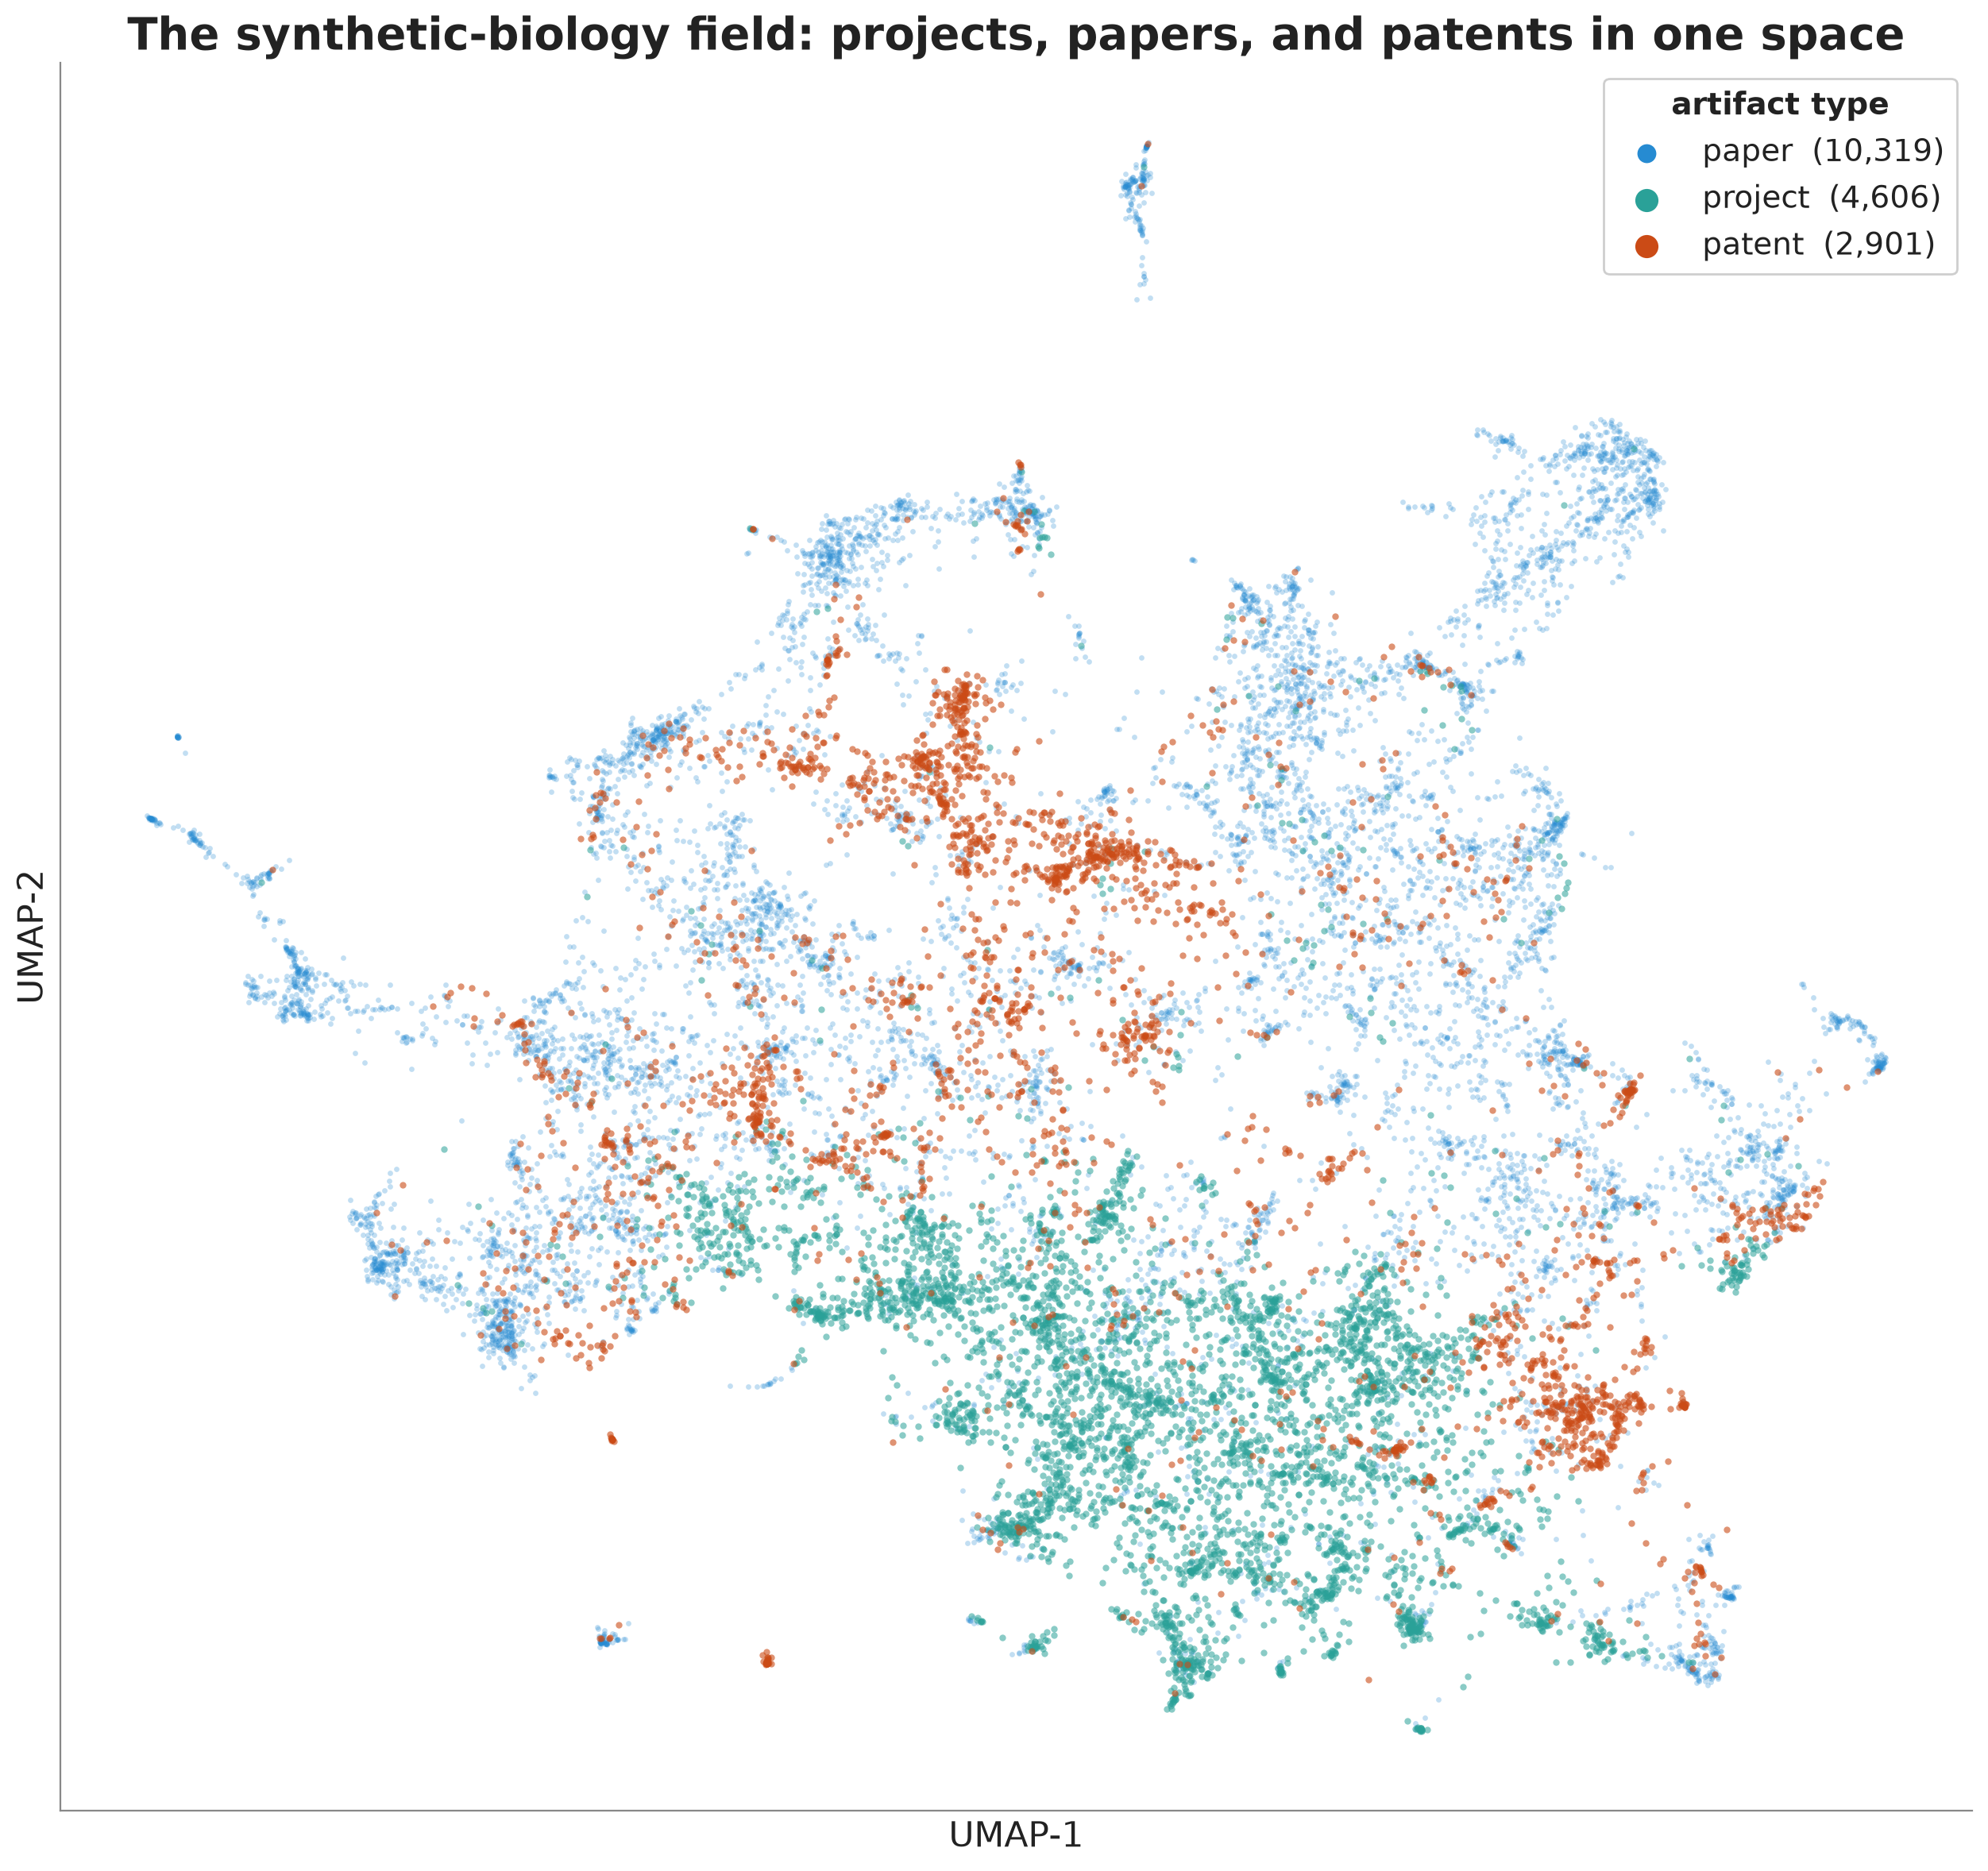
\includegraphics[width=0.92\linewidth]{tripartite_map.png}
\caption{The corpus in two dimensions. Every project, paper, and patent is a point,
placed by UMAP so that semantically similar artifacts fall near one another. Colour marks the artifact type.}
\label{fig:map}
\end{figure}

To turn the visible structure into something countable, we clustered the artifacts by topic. HDBSCAN, the method we used, groups points that crowd together densely and, just as important, leaves genuinely scattered points unassigned rather than forcing every document into a group \citep{campelloHDBSCAN2013}. This suits a corpus like ours, where some artifacts sit squarely in a well-defined topic and others fall between topics or stand alone. Run on the reduced embeddings, it found 84 clusters: dense knots of projects, papers, and patents that share a subject. A cluster here is an empirical topic, discovered from the text rather than imposed from a list, a group of documents the model judged to be about the same thing.

A cluster arrives as a numbered bag of documents with no name; naming it is where human and machine trade off. For each cluster we took the handful of documents closest to its centre, the most representative examples, and passed their titles and abstracts to a language model with one task: read these and say what they have in common. The model returned a short label and a description, which a human then checked and, where needed, corrected against the cluster's contents. Of the 84 labels, roughly 20 required correction or simplification. The failures were systematic: the centroid documents are, by definition, the most typical members of a cluster, but the outermost members can be only loosely related to that core. A label derived from the centroid sometimes described the core well but overfitted to it, using vocabulary that was accurate for the most central documents but too narrow or too specific for the artifacts that had been pulled into the cluster at its edges. Simplifying the label to a broader but still accurate description produced a name that was honest about what the whole cluster contained, not just its most representative examples. The roughly two-thirds of labels that were accepted unchanged were typically clusters with tight, well-defined cores, where the centroid documents were genuinely representative of the whole. This mirrors the project's whole method in miniature. The machine reads at a scale no person could, proposing a label from ten abstracts in a second; the human supplies the judgment to catch the cases where the model latched onto specifics that did not generalize. Neither alone would do it well.

Labelled, the map becomes legible (Figure~\ref{fig:topicmap}). The clusters range across the field: computational design tools, genetic logic circuits, biosensors, therapeutic engineering, and, in several of them, the microbial and cyanobacterial work at the heart of this thesis's case study. Each cluster carries a count of how many projects, papers, and patents it holds, which already says something. Some clusters are almost all papers, some almost all patents, and a few are dominated by student projects, a first hint that the three artifact types specialize in partly different regions of the same field.

\begin{figure}[htbp]
\centering
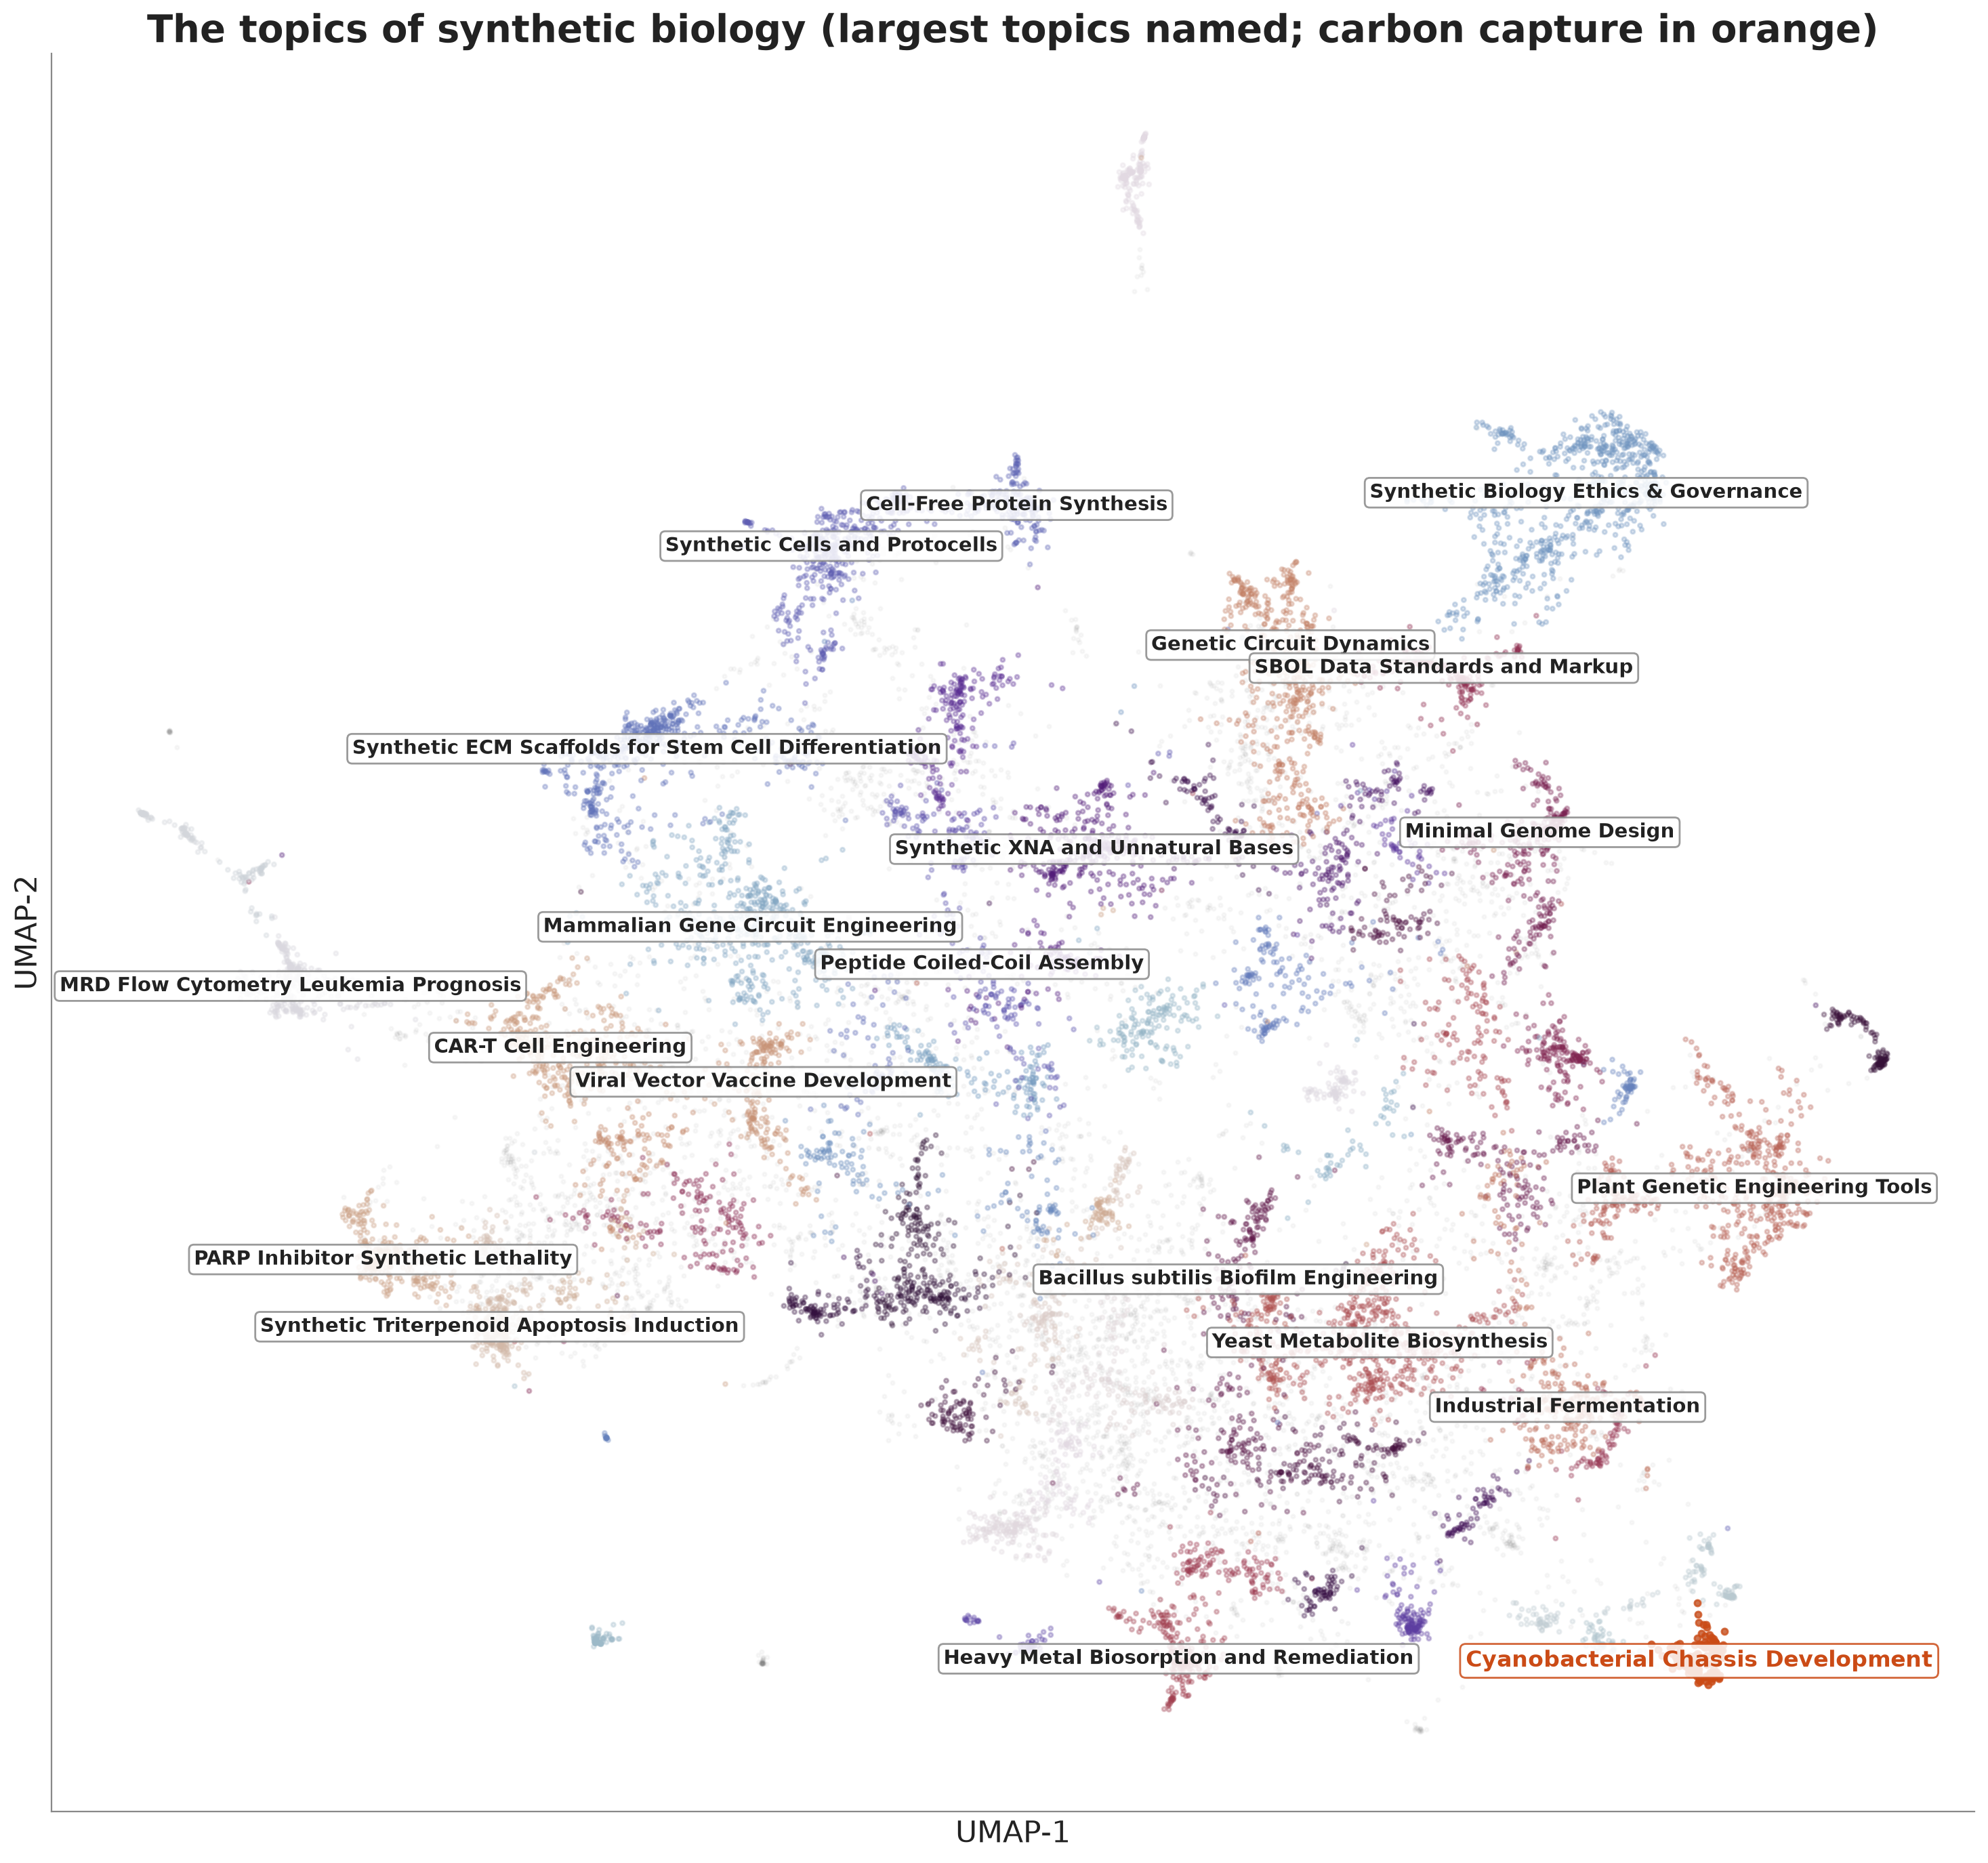
\includegraphics[width=0.92\linewidth]{tripartite_topic_map.png}
\caption{The same map, with topic clusters labelled. Each labelled region is a cluster
found by HDBSCAN and named from its most representative documents. The cyanobacterial and fermentation clusters that make up the carbon-capture case study sit close together.}
\label{fig:topicmap}
\end{figure}

\subsection{The carbon-capture slice}

This is where the case study re-enters, as a specific neighbourhood on the map. Three adjacent clusters hold the carbon-capture work, and together they trace the arc the whole thesis is about. Cluster 7, Cyanobacterial Metabolic Engineering, is dominated by student projects: 48 of its 58 documents are iGEM projects, the Uppsala team's descendants among them. Its near-neighbour cluster 8, Cyanobacterial Chassis Development, is dominated by papers, 120 of 135, the academic literature on engineering these organisms. And cluster 62, Industrial Fermentation, is overwhelmingly patents, 211 of 259 documents, the commercial work on turning waste gases into fuels and chemicals. Student projects, academic papers, and patents, sitting in three tight, adjacent clusters, arranged almost exactly along the project-to-paper-to-patent path the introduction sketched.

Finally, we tagged the carbon-capture subset and put it on the globe. Every artifact in these clusters, and others matching the case-study criteria, carries a flag marking it as carbon-capture work, so the slice can be pulled out and mapped by city.
% [FLAG: figure needed] A world map of carbon-capture cities (all three artifact types) belongs here. No such geographic figure exists yet in outputs/figures/; closest current assets are cc_city_leaderboard.png and cc_city_centrality.png (bar charts, used later in Results). Create the city map or repoint this reference.
The map shows where this work concentrates: a scatter of cities, a few of them thick with activity across all three artifact types. Uppsala is on it, unsurprisingly, along with the places the results chapter singles out as the centres of gravity for cyanobacterial carbon capture. With the corpus built, embedded, clustered, and tagged, the data is finally ready to be questioned. The next chapter does the questioning.

% ============================================================
\section{Results}
% ============================================================

The corpus is built; now we use it. This chapter asks the thesis's question of the data directly, then spends most of its length trying to break the answer. The pattern is the same throughout: propose a measure of whether a city's projects, papers, and patents are related, check what it says, and then attack it, with robustness checks on the model's assumptions, the sample, and the parameters, plus an independent validation from data that the measure never touched. What survives that treatment is what we are willing to claim.

The chapter has three movements. The first is about measurement: the obvious measure fails, and understanding why it fails leads directly to the one that works. The second is about robustness: having found a positive result, we vary everything that could have manufactured it, dropping countries, changing cluster counts, adjusting the city-depth threshold, and adding a regression and a difference-in-differences model to put the result in a form that invites comparison with the economic-geography literature. The third is about validation: we check the semantic relatedness against data from a completely different source, the physical parts students built, to confirm that the pattern exists outside the embedding space. That check is the one that removes the last legitimate worry about whether we have found something real or something our model invented.

\subsection{Project-level alignment}

Before asking about city-level structure, it is worth asking the simplest possible question of the data: is any given project semantically closer to the papers in its own city than to papers elsewhere? For each of the \statAlignNProjects{} projects with a city assignment and at least one same-city paper, we computed two numbers: the average cosine similarity between the project and all papers from the same city, and the average cosine similarity between the project and papers from a random set of other cities of the same size. The difference between these two averages is the project's local alignment: positive if the project sits closer to its own city's research than to the rest of the field, negative if it does not.

The result is clear. The mean alignment across all \statAlignNProjects{} projects is $\bar{\delta} = \statAlignMeanDelta{}$, and \statAlignFracPos{} of projects show a positive alignment. A one-sample paired $t$-test on the distribution of individual alignment scores gives $t = \statAlignT{}$ (unclustered) and $t = \statAlignTClustered{}$ when errors are clustered by city to account for the fact that projects from the same city share the same local paper environment. Both values are far beyond any conventional significance threshold. At the city level, \statAlignFracCitiesPos{} of cities show a positive mean alignment across their own projects. The effect is larger in cities with more documents: the mean alignment for large cities (above the median paper count) is $\statAlignDeltaLarge{}$, versus $\statAlignDeltaSmall{}$ for small ones ($t = \statAlignTCity{}$ at the city level). Larger cities have richer local paper environments that provide a more sharply defined semantic neighborhood, so their projects have more room to align locally rather than to the global average.

This is the most direct test of the thesis's central claim, and it passes clearly. At the level of individual projects, the average project in our corpus sits semantically closer to its own city's research than to research from other cities, by a small but highly consistent margin. The finding sets the stage for the city-level analyses that follow, which ask not just whether local alignment exists, but how to measure it in a way that is robust to city size and independent of the specific embedding model.

The first measure is the natural one. For each city $c$, let $P_c$ be its set of projects and $Q_c$ its set of papers. The centroid of the projects is the average embedding:
\begin{equation}
  \bar{\mathbf{p}}_c = \frac{1}{|P_c|} \sum_{i \in P_c} \mathbf{e}_i
\end{equation}
where $\mathbf{e}_i \in \mathbb{R}^{768}$ is the embedding of document $i$. The paper centroid $\bar{\mathbf{q}}_c$ is defined the same way. We then measure the angle between these two vectors using cosine similarity:
\begin{equation}
  \text{sim}(\bar{\mathbf{p}}_c, \bar{\mathbf{q}}_c)
  = \frac{\bar{\mathbf{p}}_c \cdot \bar{\mathbf{q}}_c}
         {\|\bar{\mathbf{p}}_c\| \, \|\bar{\mathbf{q}}_c\|}
\end{equation}
This ranges from $-1$ (perfect opposition in meaning) to $+1$ (perfect alignment), with $0$ denoting no consistent directional relationship. Cosine similarity is standard for high-dimensional embeddings because it ignores vector magnitude and focuses on orientation: two documents that are both about cyanobacteria will point in roughly the same direction through the 768-dimensional space, whatever their lengths or styles. It is also what SPECTER2 was trained to optimize for citation prediction, so the geometry the model learned is exactly what cosine similarity reads. Computed across all cities with enough documents in both corpora, the mean similarity is \statOverlapMean{} and the median is
\statOverlapMedian{}, on a scale where 1 is identical. Taken at face value, this looks
like a resounding yes: almost every city's students and academics are pointing at the same part of conceptual space.

It is too good, and it does not survive a second look. The centroids are high everywhere, including for city pairs that share no obvious subject, which signals that the measure is picking up something other than local relatedness. When we regress the overlap on the log of each city's document count:
\begin{equation}
  \text{sim}(\bar{\mathbf{p}}_c, \bar{\mathbf{q}}_c)
  = \alpha + \beta_1 \log|P_c| + \beta_2 \log|Q_c| + \epsilon_c
\end{equation}
size dominates: overlap correlates at \statSizePapersR{} with paper count and
\statSizeProjectsR{} with project count (Figure~\ref{fig:centroidsize}). The mechanism is
a known property of high-dimensional averaging, sometimes called centroid collapse. Each document's embedding lives in a large space with a dense cluster near the origin, the region where all of a field's general vocabulary concentrates. As a city accumulates more documents, its centroid is pulled steadily toward that dense centre, where the generic vocabulary of all of synthetic biology overlaps. Large cities end up with centroids near each other and near the global mean, not because their students and academics work on the same things, but because averaging across a large, mixed corpus washes away the specificity that would distinguish one city's focus from another's. The effect runs equally for cities with genuinely aligned projects and papers and for cities whose students and academics work in entirely different subfields: both compress to the same semantic centre as the corpus grows. The centroid measure is a size artifact. It answers a question about how much a city publishes, dressed up as a question about what it publishes. This was the first real result of the project, and it was a negative one — but a useful one, because the mechanism pointed directly at the fix.

\begin{figure}[htbp]
\centering

\includegraphics[width=0.85\linewidth]{centroid_size_artifact.png}
\caption{Why the centroid measure fails. Project-to-paper centroid overlap climbs with the
number of documents a city has, so the measure mostly tracks city size rather than local relatedness.}
\label{fig:centroidsize}
\end{figure}

The failure of the centroid measure points at its own fix. The problem was averaging: it collapses a city's entire research output into one point and loses the specificity of what it works on. The fix is to stop averaging and start counting topics. Instead of representing a city as a single vector, we represent it as a profile across the 84 clusters from the previous chapter: for each cluster, how many of the city's documents fall into it? A city is now a distribution over topics rather than a point in space. Relatedness becomes a sharper question: not do the city's students and academics point in roughly the same direction on average, but do they specifically co-invest in the same narrow subjects? A city might be enormous and productive across every topic in the field, earning a high centroid similarity with everyone, while its students and academics work on entirely different subfields. The topic-profile approach distinguishes that case from a city where both groups genuinely concentrate on the same handful of clusters. That distinction is the one the thesis is built to make.

The measure built on this is deliberately simple, and deliberately free of averaging. For city $c$, let $T_{\text{proj}}(c)$ be the set of clusters containing at least one of the city's projects, and $T_{\text{paper}}(c)$ the set containing at least one of its papers. The topic overlap is:
\begin{equation}
  O(c) = \frac{\left|T_{\text{proj}}(c) \cap T_{\text{paper}}(c)\right|}
              {\left|T_{\text{proj}}(c) \cup T_{\text{paper}}(c)\right|}
\end{equation}
This is the Jaccard similarity between the two topic sets. It ranges from 0 (no shared topics whatsoever) to 1 (every topic the students touch, the academics also touch), and the denominator controls for breadth: a city that covers 50 topics in each type gets no credit simply for covering the field widely, since the denominator grows with the union. A city whose students and academics both work on cyanobacterial metabolic engineering, genetic circuits, and biosensors scores high; a city whose students focus on food engineering while its academics publish on therapeutic proteins scores low, even if both groups are equally productive. The measure is insensitive to size in a way the centroid is not, because it counts topics rather than averaging representations. We restrict the comparison to cities with at least \statClusterMinDocs{} documents of each type, which leaves
\statClusterNCitiesDense{} cities with profiles dense enough to be reliable. Averaged across
them, a city's projects and papers share a topic about six percent of the time. That raw fraction means nothing until it is held against a baseline, and building the right baseline is the whole analytical game.

That baseline is borrowed from revealed-relatedness logic in economic geography: two things are genuinely related if they appear together more than chance predicts; here, a city's projects and papers are genuinely related if they share topics more than size and topic popularity alone can produce. To construct the null, we run a permutation test. We fix each city's paper topic set and randomly reassign its project set to another city, drawing without replacement across the full set of $\statClusterNCitiesDense{}$ cities, then recompute the mean overlap $\bar{O}$ across all cities. We repeat this $B = 10{,}000$ times. Each shuffle preserves the marginal distributions: every city keeps exactly as many projects and papers as before, and every cluster retains exactly as many members, so any excess that survives the shuffle must come from the specific co-location of topics, not from size or cluster popularity. Formally, the test statistic and its $p$-value are:
\begin{equation}
  \hat{\Delta} = \bar{O}_{\text{obs}} - \frac{1}{B}\sum_{b=1}^{B} \bar{O}_{(b)}, \qquad
  p = \frac{1}{B}\left|\left\{b : \bar{O}_{(b)} \geq \bar{O}_{\text{obs}}\right\}\right|
\end{equation}
The real cities beat the null: the observed mean overlap is \statClusterPermObserved{}, against a shuffled average of \statClusterPermNullMean{}, an excess of
\statClusterPermExcess{} ($p = \statClusterPermP{}$), shown in Figure~\ref{fig:perm}.
The entire distribution of 10,000 shuffled means sits below the observed value. Once city size and topic popularity are held fixed, a city's student projects and its academic papers share specific topics more often than chance allows. That is the thesis's central positive result.

\begin{figure}[htbp]
\centering
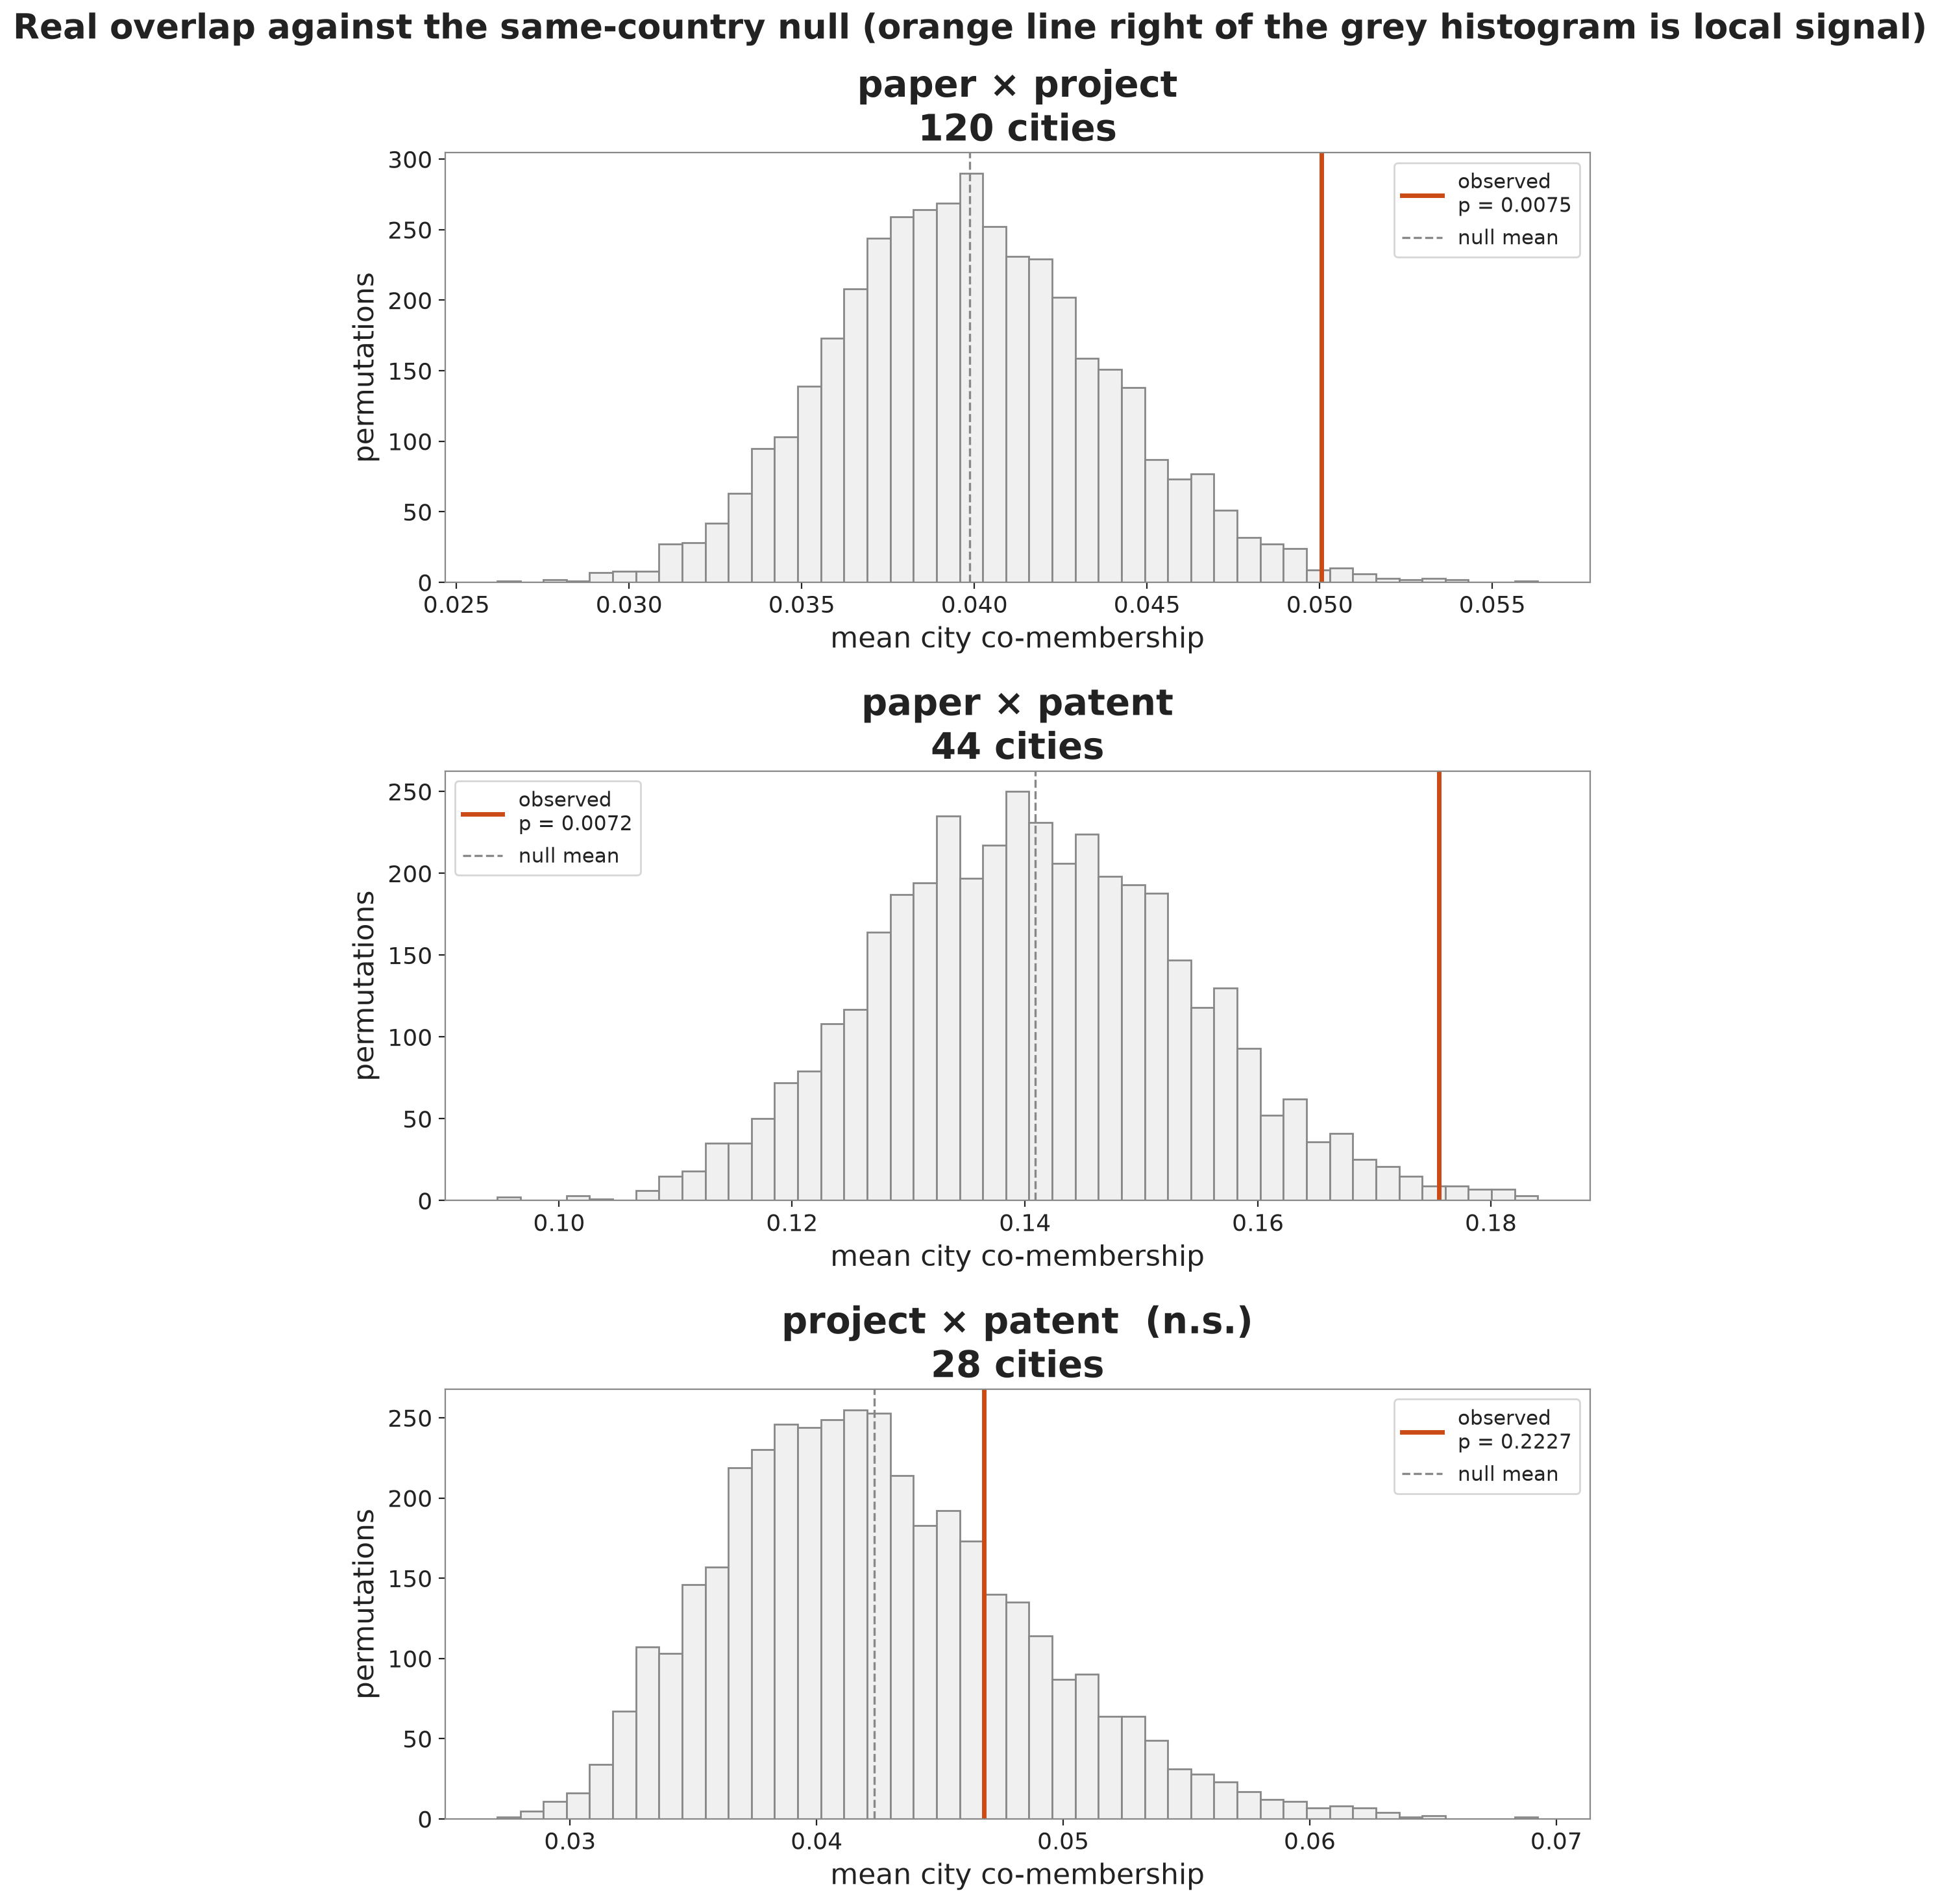
\includegraphics[width=0.85\linewidth]{tripartite_permutation.png}
\caption{The central result. The observed rate at which a city's projects and papers share
topics (marked line) sits far above the distribution produced by reshuffling projects across cities (histogram), which holds city size and topic popularity fixed. The gap is the size-independent local relatedness.}
\label{fig:perm}
\end{figure}

A single positive result, however clean, is a hypothesis until it has been attacked. The permutation test rules out size and topic popularity as explanations, but it rests on a set of choices that were made before the test was run: which countries are in the sample, how many clusters the HDBSCAN run produced, and how deep a city's corpus needs to be before it is included. Any one of these could, in principle, have manufactured the result: a particular country might drive it all, a particular cluster count might produce an artificial excess, a particular depth threshold might include only the cities with coincidentally aligned corpora. For the result to be taken seriously, it needs to survive all of these checks, not just one. So we varied each in turn and watched whether the excess held. The three checks that follow are not supplementary analyses; they are the conditions that turn a positive test into a credible finding.

The first worry is that one country carries the whole effect. If a large national system concentrates its iGEM activity and its academic output onto the same few topics, that national pattern could masquerade as a city-level effect: the excess in the permutation test would reflect national specialization, not local relatedness within cities. To check, we ran a leave-one-country-out analysis. We dropped each country from the sample in turn, recomputed the permutation test on the remaining cities, and recorded the excess (Figure~\ref{fig:leavecountry}). The result barely moves across all exclusions. Removing the United States, which supplies a large share of both iGEM teams and synthetic-biology papers, leaves the excess essentially unchanged. Removing China, which supplies the largest number of iGEM teams in recent years, leaves it essentially unchanged. No single country, however large, drives the result: the relatedness is distributed across the sample rather than concentrated in one national system. A claim about cities in general needs exactly this: if it survives with any one country removed, it is not being held up by a single country's peculiarities.

\begin{figure}[htbp]
\centering
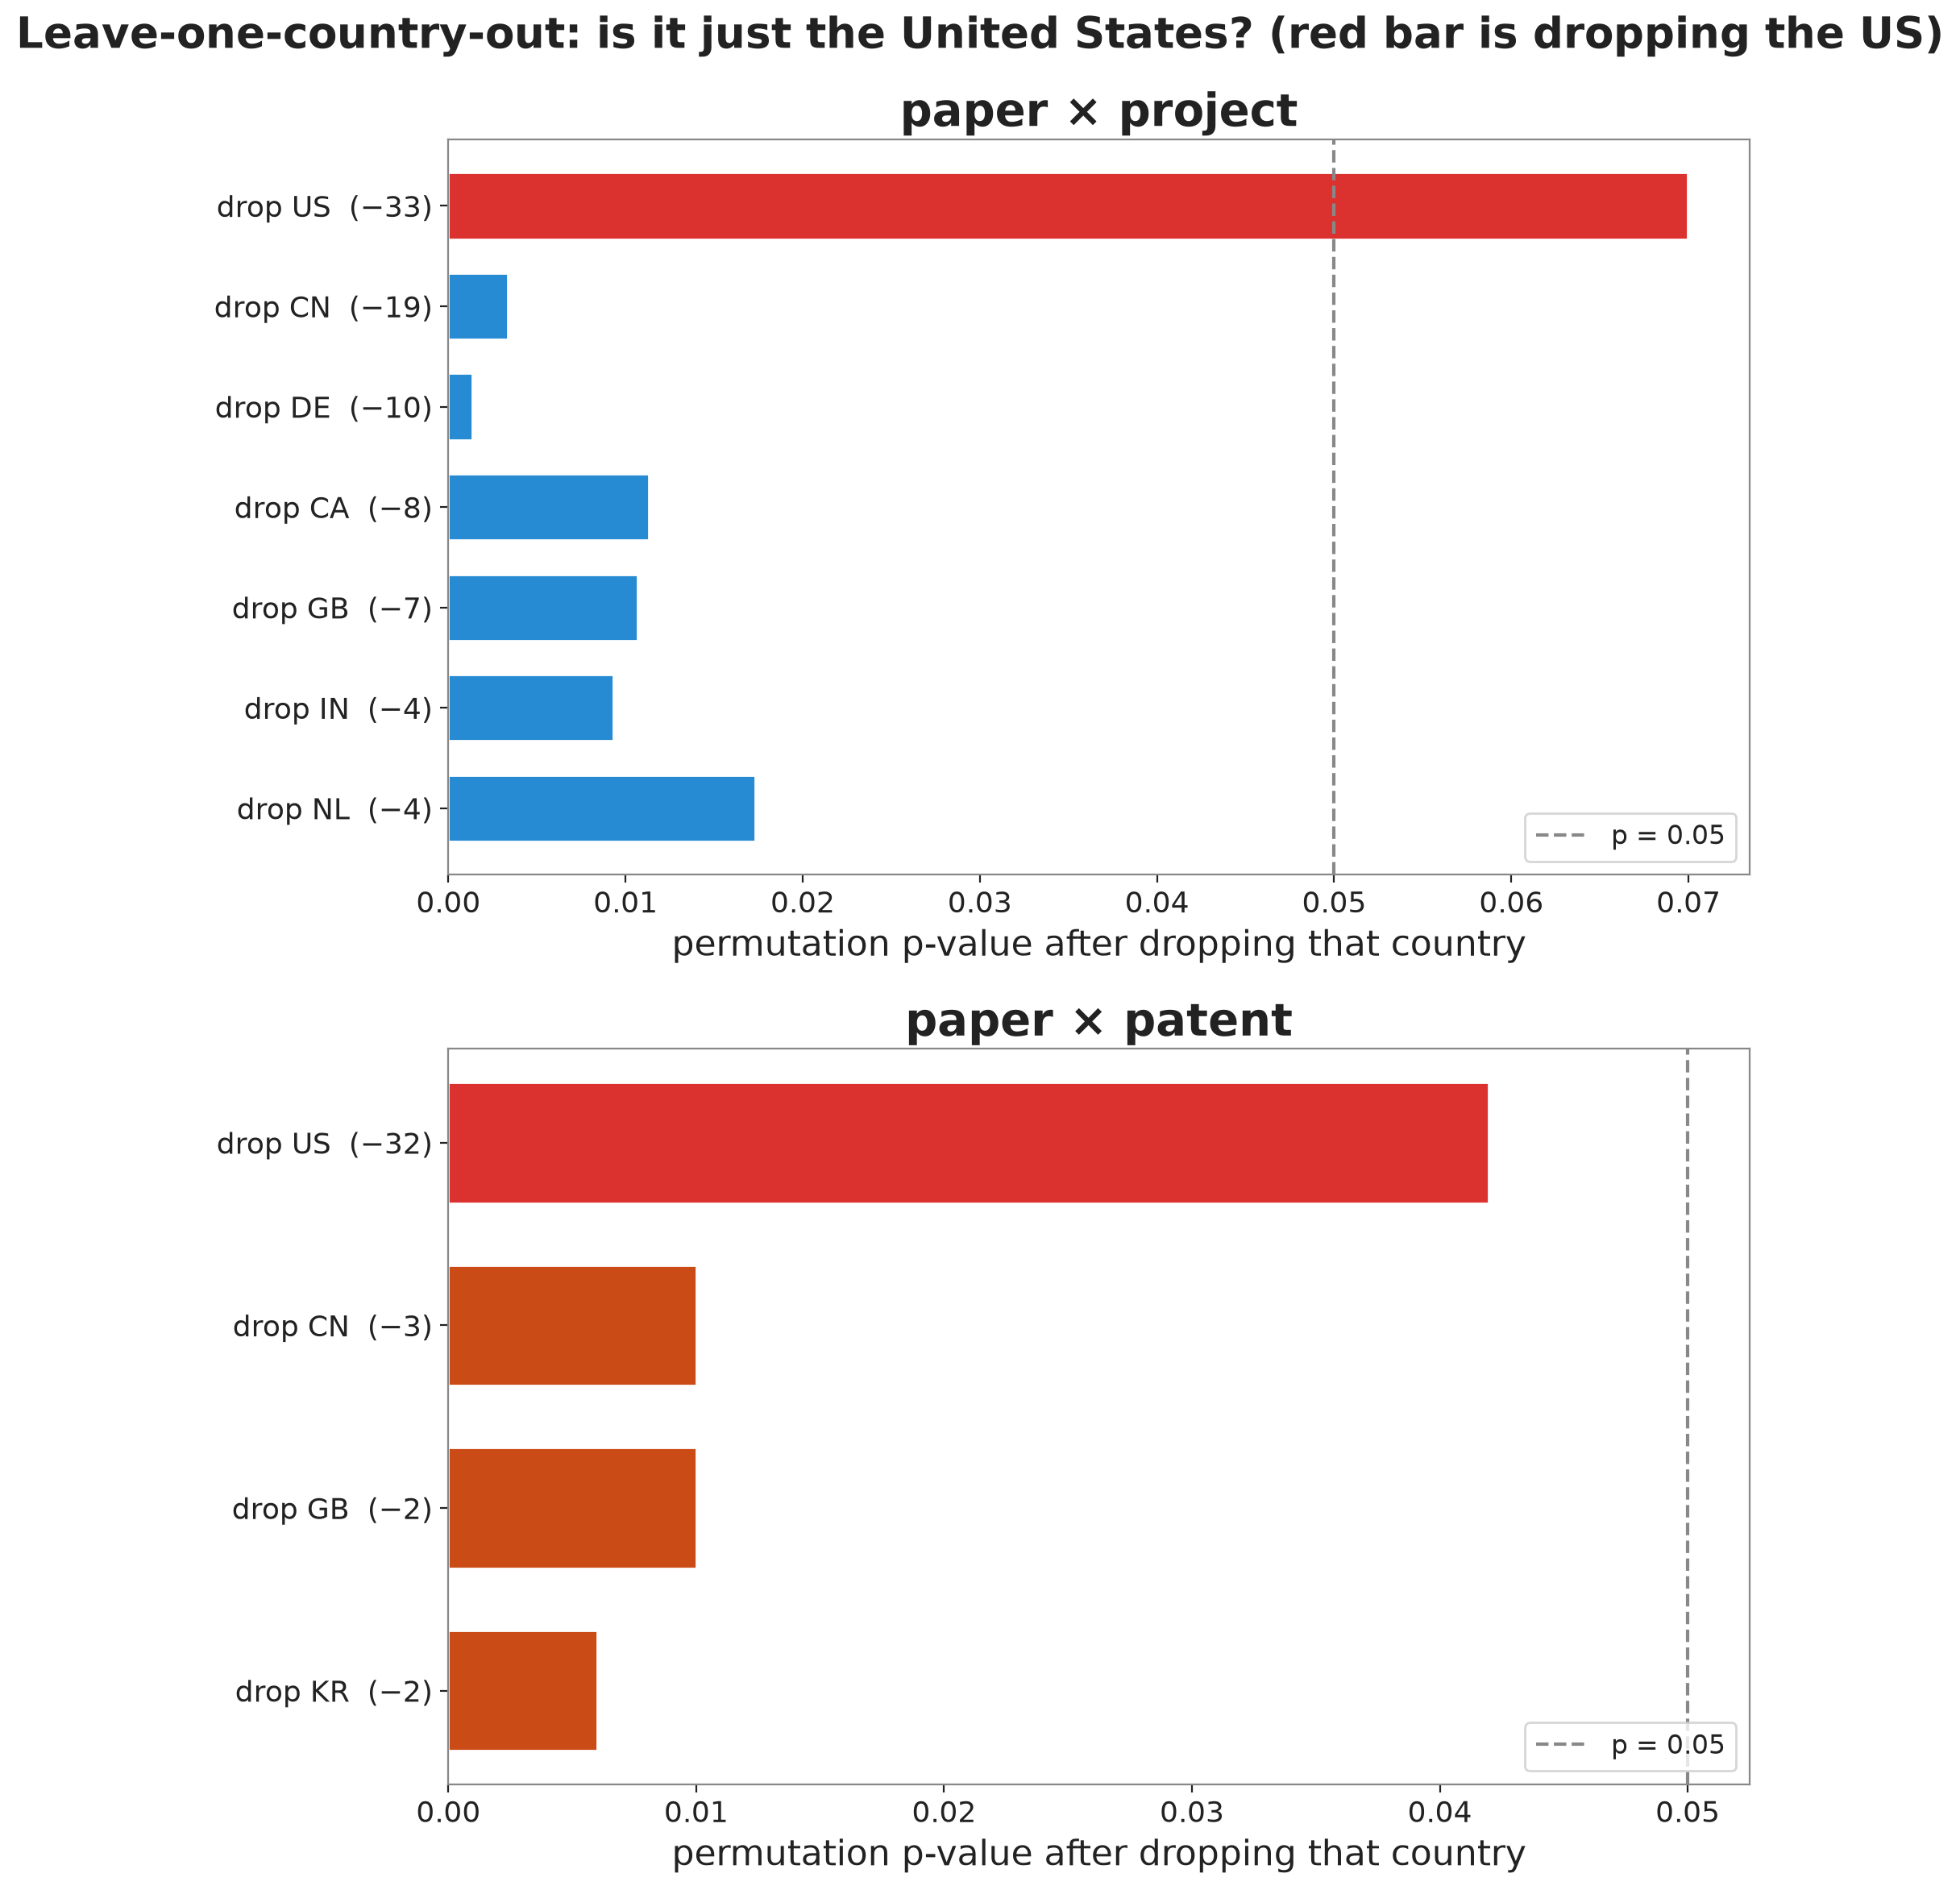
\includegraphics[width=0.85\linewidth]{robust_leave_country.png}
\caption{Leave-one-country-out. Recomputing the excess with each country removed in turn
leaves it essentially unchanged; no single national system drives the result.}
\label{fig:leavecountry}
\end{figure}

The second worry is the clustering itself. The 84 topics came from one run of HDBSCAN with one set of parameters; a different number of clusters could, in principle, tell a different story. The concern runs in both directions. Very fine clusters split each subject into many tiny pieces, making it rare for any city's projects and papers to land in the same narrow bin, which would mechanically suppress the excess. Very coarse clusters lump everything into a few broad subjects, making it easy for any city to score well on overlap, which would inflate the excess across the board. Either regime could manufacture or erase the effect independently of whether local relatedness is real.

To check, we replaced the semantic HDBSCAN clusters with $k$-means at a range of resolutions, sweeping $k$ from fine to coarse, and recomputed the permutation excess at each value (Figure~\ref{fig:kcurve}). The excess persists across the sweep. It shrinks when the clusters are very fine, as expected once topic-sharing becomes rare for everyone, but it stays positive and significant at every reasonable resolution and never approaches zero until the clusters are thin enough that the test loses power entirely. The result does not depend on one lucky choice of cluster count. Whatever the granularity at which we carve up the field, a city's students and academics specialize in the same corners of it more than size and topic popularity can account for.

\begin{figure}[htbp]
\centering

\includegraphics[width=0.85\linewidth]{robust_kcurve.png}
\caption{Varying the number of topics. The size-independent excess stays positive and
significant across a wide sweep of cluster counts, shrinking only when clusters become very fine.}
\label{fig:kcurve}
\end{figure}

The third worry is the depth threshold. We required at least \statClusterMinDocs{} documents of each type per city, and one might ask whether the effect lives only in a small set of unusually deep cities, or depends on exactly where the threshold was drawn. A high threshold keeps only the largest, most specialized cities; a low threshold lets in smaller cities with noisier topic profiles. Either could bias the result: high-threshold cities are more likely to have stable topic profiles that align by chance in large fields, and low-threshold cities introduce noise that could suppress the excess. We swept the threshold across a wide range, recomputing the excess at each setting (Figure~\ref{fig:power}). The excess persists across the range. Deeper cities, those above the higher thresholds, show the effect more cleanly, as one would expect when each city's topic profile is measured from more documents and is therefore more reliable. But the effect is not manufactured by the threshold: it appears at low thresholds among shallow cities and grows larger as the data get richer, which is the pattern a real signal leaves. A spurious result would not reliably strengthen as measurement improves. Taken together, the three checks establish that the central result does not rest on any particular feature of the sample, the clustering, or the inclusion criteria.

\begin{figure}[htbp]
\centering

\includegraphics[width=0.85\linewidth]{robust_power.png}
\caption{Varying the document threshold. As the minimum documents per city is raised and
lowered, the excess persists, and shows more cleanly in the deeper cities.}
\label{fig:power}
\end{figure}

The permutation test answers whether the excess is real; ordinary least squares gives its magnitude next to observable confounders and lets us report it in the language reviewers expect. We fit:
\begin{equation}
  O_c = \alpha + \beta_1 \log N_{\text{proj},c}
              + \beta_2 \log N_{\text{paper},c}
              + \sum_{k} \gamma_k \,\mathbb{1}[c \in \text{country}\,k]
              + \epsilon_c
\end{equation}
where $O_c$ is city $c$'s project-to-paper Jaccard overlap, $N_{\text{proj},c}$ and $N_{\text{paper},c}$ are its project and paper counts on a log scale (size effects are multiplicative, so log transformation is appropriate), and the $\gamma_k$ are country fixed effects that absorb any national-level systematic differences in how much countries specialize or how thoroughly they are covered by the iGEM and OpenAlex data. The contrast with the centroid regression is the headline (Table~\ref{tab:ols}). For the centroid measure, the size coefficients dominate: the regression $R^2$ is \statOlsRsqModelOne{} and size explains most of it. For the cluster overlap, the paper-count and project-count coefficients are small and statistically weak ($p = \statClusterSizePapersP{}$ and $p = \statClusterSizeProjectsP{}$), and the total $R^2$ is only \statClusterOlsRsq{}. Moving from averages to topic profiles has stripped out the size artifact by construction. The Jaccard denominator grows with the union of topics covered, so a large city that covers the whole field earns no more overlap credit than a focused city working on a narrow subfield. The residual variation in $O_c$, the part neither size nor country absorbs, is the city-level variation in topical alignment that the permutation test showed is real.

\begin{table}[htbp]
\centering
\caption{Size explains the centroid measure but not the cluster measure. City size dominates
the centroid-overlap regression and all but vanishes once relatedness is measured as shared topic clusters.}
\label{tab:ols}
\begin{tabular}{lcc}
\toprule
Measure & Model $R^2$ & Size significance \\
\midrule
Centroid overlap & \statOlsRsqModelOne{} & $p < 10^{-7}$ \\
Cluster-topic overlap & \statClusterOlsRsq{} & $p = \statClusterSizePapersP{},\ \statClusterSizeProjectsP{}$ \\
\bottomrule
\end{tabular}
\end{table}

The coefficients deserve to be read in substantive terms, not only as significance test outcomes. The near-zero size coefficients in the cluster-overlap regression confirm what the permutation test showed: once relatedness is measured as topic co-membership rather than centroid similarity, city volume has almost no explanatory power. The residual variation in $O_c$ — the part neither size nor country explains — is interpretable as city-idiosyncratic topical alignment, the tendency of a particular place to concentrate its student and academic synthetic biology onto the same narrow corners of the field. The total $R^2$ of \statClusterOlsRsq{} means that most of that variation is genuinely unexplained by the controls we include, which is expected: the model is not trying to predict what cities do, only to show that size and national context do not account for what the permutation test already found. A city-level fixed-effects analysis, had we panel data over many periods, would absorb city-specific standing specialization as well; the cross-sectional OLS with country effects is the appropriate specification for a single-wave analysis of this kind.

The cross-sectional regression shows that alignment exists; it cannot say whether it is a living year-to-year coupling or a structural feature baked into each city's long-run specialization. A difference-in-differences design separates the two. We split the sample into five-year periods and ask, within a city and topic, whether rising project activity in one period is accompanied by rising paper activity. Specifically, let $Y_{c,k,t}$ be the paper share of cluster $k$ in city $c$ in period $t$ (fraction of the city's papers landing in that cluster), and $X_{c,k,t}$ the corresponding project share. We fit:
\begin{equation}
  Y_{c,k,t} = \alpha_c + \delta_{k,t} + \beta\, X_{c,k,t} + \epsilon_{c,k,t}
\end{equation}
where $\alpha_c$ is a city fixed effect, absorbing each city's standing topic profile across all periods; $\delta_{k,t}$ is a topic-by-period effect, absorbing how popular cluster $k$ is in period $t$ across all cities; and $\beta$ captures the residual within-city, within-topic co-movement that remains after both are differenced out. Standard errors are clustered by city, since the city-cluster-period observations within a city share common shocks. The estimate is $\hat{\beta} = \statDidEstimate{}$ ($t = \statDidTClustered{}$, across \statDidNCities{} cities and 84 topics), positive and significant but small (Figure~\ref{fig:did}). The coefficient is in the units of both variables, which are fractions: if a city's project share in a given topic rises by one percentage point above its own baseline in a period, its paper share in that topic rises by approximately $\statDidEstimate{}$ percentage points above its own baseline in the same period, after the topic-period trend is removed. The magnitude is small because the city and topic-period fixed effects absorb most of the variation in paper shares; what $\hat\beta$ captures is the dynamic residual, the portion of year-to-year co-movement that is not accounted for by where a city already specializes or where the field is trending globally. A coefficient of this size, on a fraction-of-papers outcome variable, is consistent with a real but modest coupling between project activity and academic output within the same topic window. It is not the main story, which is structural, but it rules out the possibility that the cross-sectional alignment is purely historical and never updates.

The interpretation is precise. By differencing out the city baseline, we remove the standing specialization that accounts for most of the permutation-test signal. What remains is a smaller but real dynamic component: when a city's students push into a topic in one period, its academic output in that same topic rises slightly. The large structural signal is about cities with persistent dual investment in a subfield; this smaller dynamic signal says that coupling is also updated year to year.

\begin{figure}[htbp]
\centering

\includegraphics[width=0.85\linewidth]{did_alignment.png}
\caption{Difference-in-differences. Within a city and topic, rising project activity is
accompanied by a small but significant rise in paper activity, once each city's baseline and each topic's trend are differenced out. The alignment is mostly standing specialization, with a smaller year-to-year component.}
\label{fig:did}
\end{figure}

\subsection{Lead-lag structure}

The difference-in-differences result found a small dynamic coupling from one period to the next. A natural follow-up is whether that coupling has a preferred direction: do student projects tend to precede academic papers in the same subfield, or the reverse, and by how long? To probe this, we ran a lead-lag analysis across the city-topic cells with enough observations to fit a trend. For each lag $\ell$ (ranging from $-5$ to $+5$ years), we computed the average cosine similarity between a city's project activity in a topic at time $t$ and its paper activity in the same topic at time $t + \ell$. A positive $\ell$ means we are comparing projects against papers that come \textit{after} the projects; a negative $\ell$ means papers that come \textit{before}. The similarity at each lag summarizes how well aligned project and paper activity is when offset by that many years.

The alignment peaks at $\ell = \statLeadlagBestLag{}$ years, reaching a mean similarity of
\statLeadlagBestSim{}. The curve is asymmetric: similarity rises from negative lags, peaks
at $+3$, and falls off for larger positive lags. The reading is careful. This is not a causal estimate; a peak at $+3$ years means that project and paper activity are most aligned when the papers are three years newer than the projects, which is consistent with a sequence in which students work on a topic a few years before the academic literature in that topic peaks locally. It is also consistent with a city whose students and academics respond in sequence to the same external stimulus, or with a city where both draw on a mentor population that shifts its focus in a way that reaches students before it shows up in publications. The peak at $+3$ years is a correlation structure, not a causal chain, but it is a plausible correlation structure for the story the thesis tells: students at the front of a local research wave, with papers consolidating behind them.

Every result so far lives inside the semantic space, which invites one deep objection: what if the whole thing is an artifact of how SPECTER2 reads text? The model was trained on scientific abstracts, and it has learned, in ways we cannot fully interpret, to organize documents by their conceptual proximity. If it has learned a systematic bias, and the overlap measure simply reflects that bias, then all of our robustness checks would agree with each other for purely internal reasons, and we would have found nothing except a property of the model. The only clean way to rule this out is to check the semantic relatedness against something the model never touched.

The BioBricks give us exactly that. The iGEM parts registry records not only the sequence and description of each part but its functional class: promoter, coding sequence, reporter, terminator, RBS (ribosome binding site), composite, and so on. A city's students leave a fingerprint in the registry: the mix of part classes they built and deposited over the years. This fingerprint is made from physical genetic components and functional annotations, not from any language the model could have read. A city that focuses on regulated gene expression deposits many promoters and RBS elements; one focused on biosensors deposits reporters; one focused on whole-pathway engineering deposits composite parts. The class distribution is a parallel description of a city's research orientation, derived from entirely different data.

The question is whether two completely different descriptions of the same cities agree. On the semantic side, we compute a city-by-city dissimilarity matrix $D^{(1)}$ in which entry $(i,j)$ is $1 - O(i,j)$, one minus the Jaccard overlap between city $i$'s and city $j$'s topic profiles across projects, papers, and patents. On the parts side, we compute a second matrix $D^{(2)}$ in which entry $(i,j)$ is the cosine distance between city $i$'s and city $j$'s BioBrick class vectors, where a class vector records how many of that city's parts are promoters, coding sequences, reporters, terminators, and so on. The two matrices describe the same cities but are built from entirely separate data sources. The Mantel statistic is the Pearson correlation between the off-diagonal entries of the two matrices:
\begin{equation}
  r_M
  = \frac{\displaystyle\sum_{i<j}
    \bigl(D^{(1)}_{ij} - \bar{D}^{(1)}\bigr)\bigl(D^{(2)}_{ij} - \bar{D}^{(2)}\bigr)}
  {\displaystyle\sqrt{
    \sum_{i<j}\!\bigl(D^{(1)}_{ij}-\bar{D}^{(1)}\bigr)^2
    \cdot
    \sum_{i<j}\!\bigl(D^{(2)}_{ij}-\bar{D}^{(2)}\bigr)^2
  }}
\end{equation}
Because the entries of a distance matrix are not independent (each city appears in many pairs), standard Pearson significance tests are invalid. The Mantel test permutes the row and column labels of one matrix, recomputing $r_M$ from scratch for each permutation, and judges the observed value against that empirical null distribution. If the semantic structure were a product of SPECTER2's geometry rather than a real feature of the cities, it would bear no relationship to the parts, which the model never saw.

They line up (Figure~\ref{fig:mantel}). Across the \statMantelNCities{} cities with enough data in both registers, $r_M = \statMantelR{}$ ($p = \statMantelP{}$): cities whose students build similar mixes of genetic parts also tend to have similar topic profiles across their projects, papers, and patents. The magnitude is moderate, which is honest and expected. BioBrick class vectors describe the physical toolkit a city's students used, which is related to but not identical with the topical subjects those students wrote about. A city that builds a lot of promoters is likely working on regulated gene expression, but the same promoter types show up across many different biological applications, so the two measures can agree on broad similarity while disagreeing on specifics. A correlation of
\statMantelR{} between such loosely coupled data sources is a meaningful signal, not a weak
one. More to the point, it comes from two independent windows onto the same cities: one built from titles and abstracts processed by a language model, one built from functional labels on deposited DNA sequences that the language model never touched. A structure imposed by SPECTER2 on text would have no reason to match the distribution of promoters and coding sequences across cities. The fact that it does is the strongest single piece of evidence in this thesis that the semantic relatedness is anchored in something real, and not merely in the model's particular way of reading a sentence.

\begin{figure}[htbp]
\centering
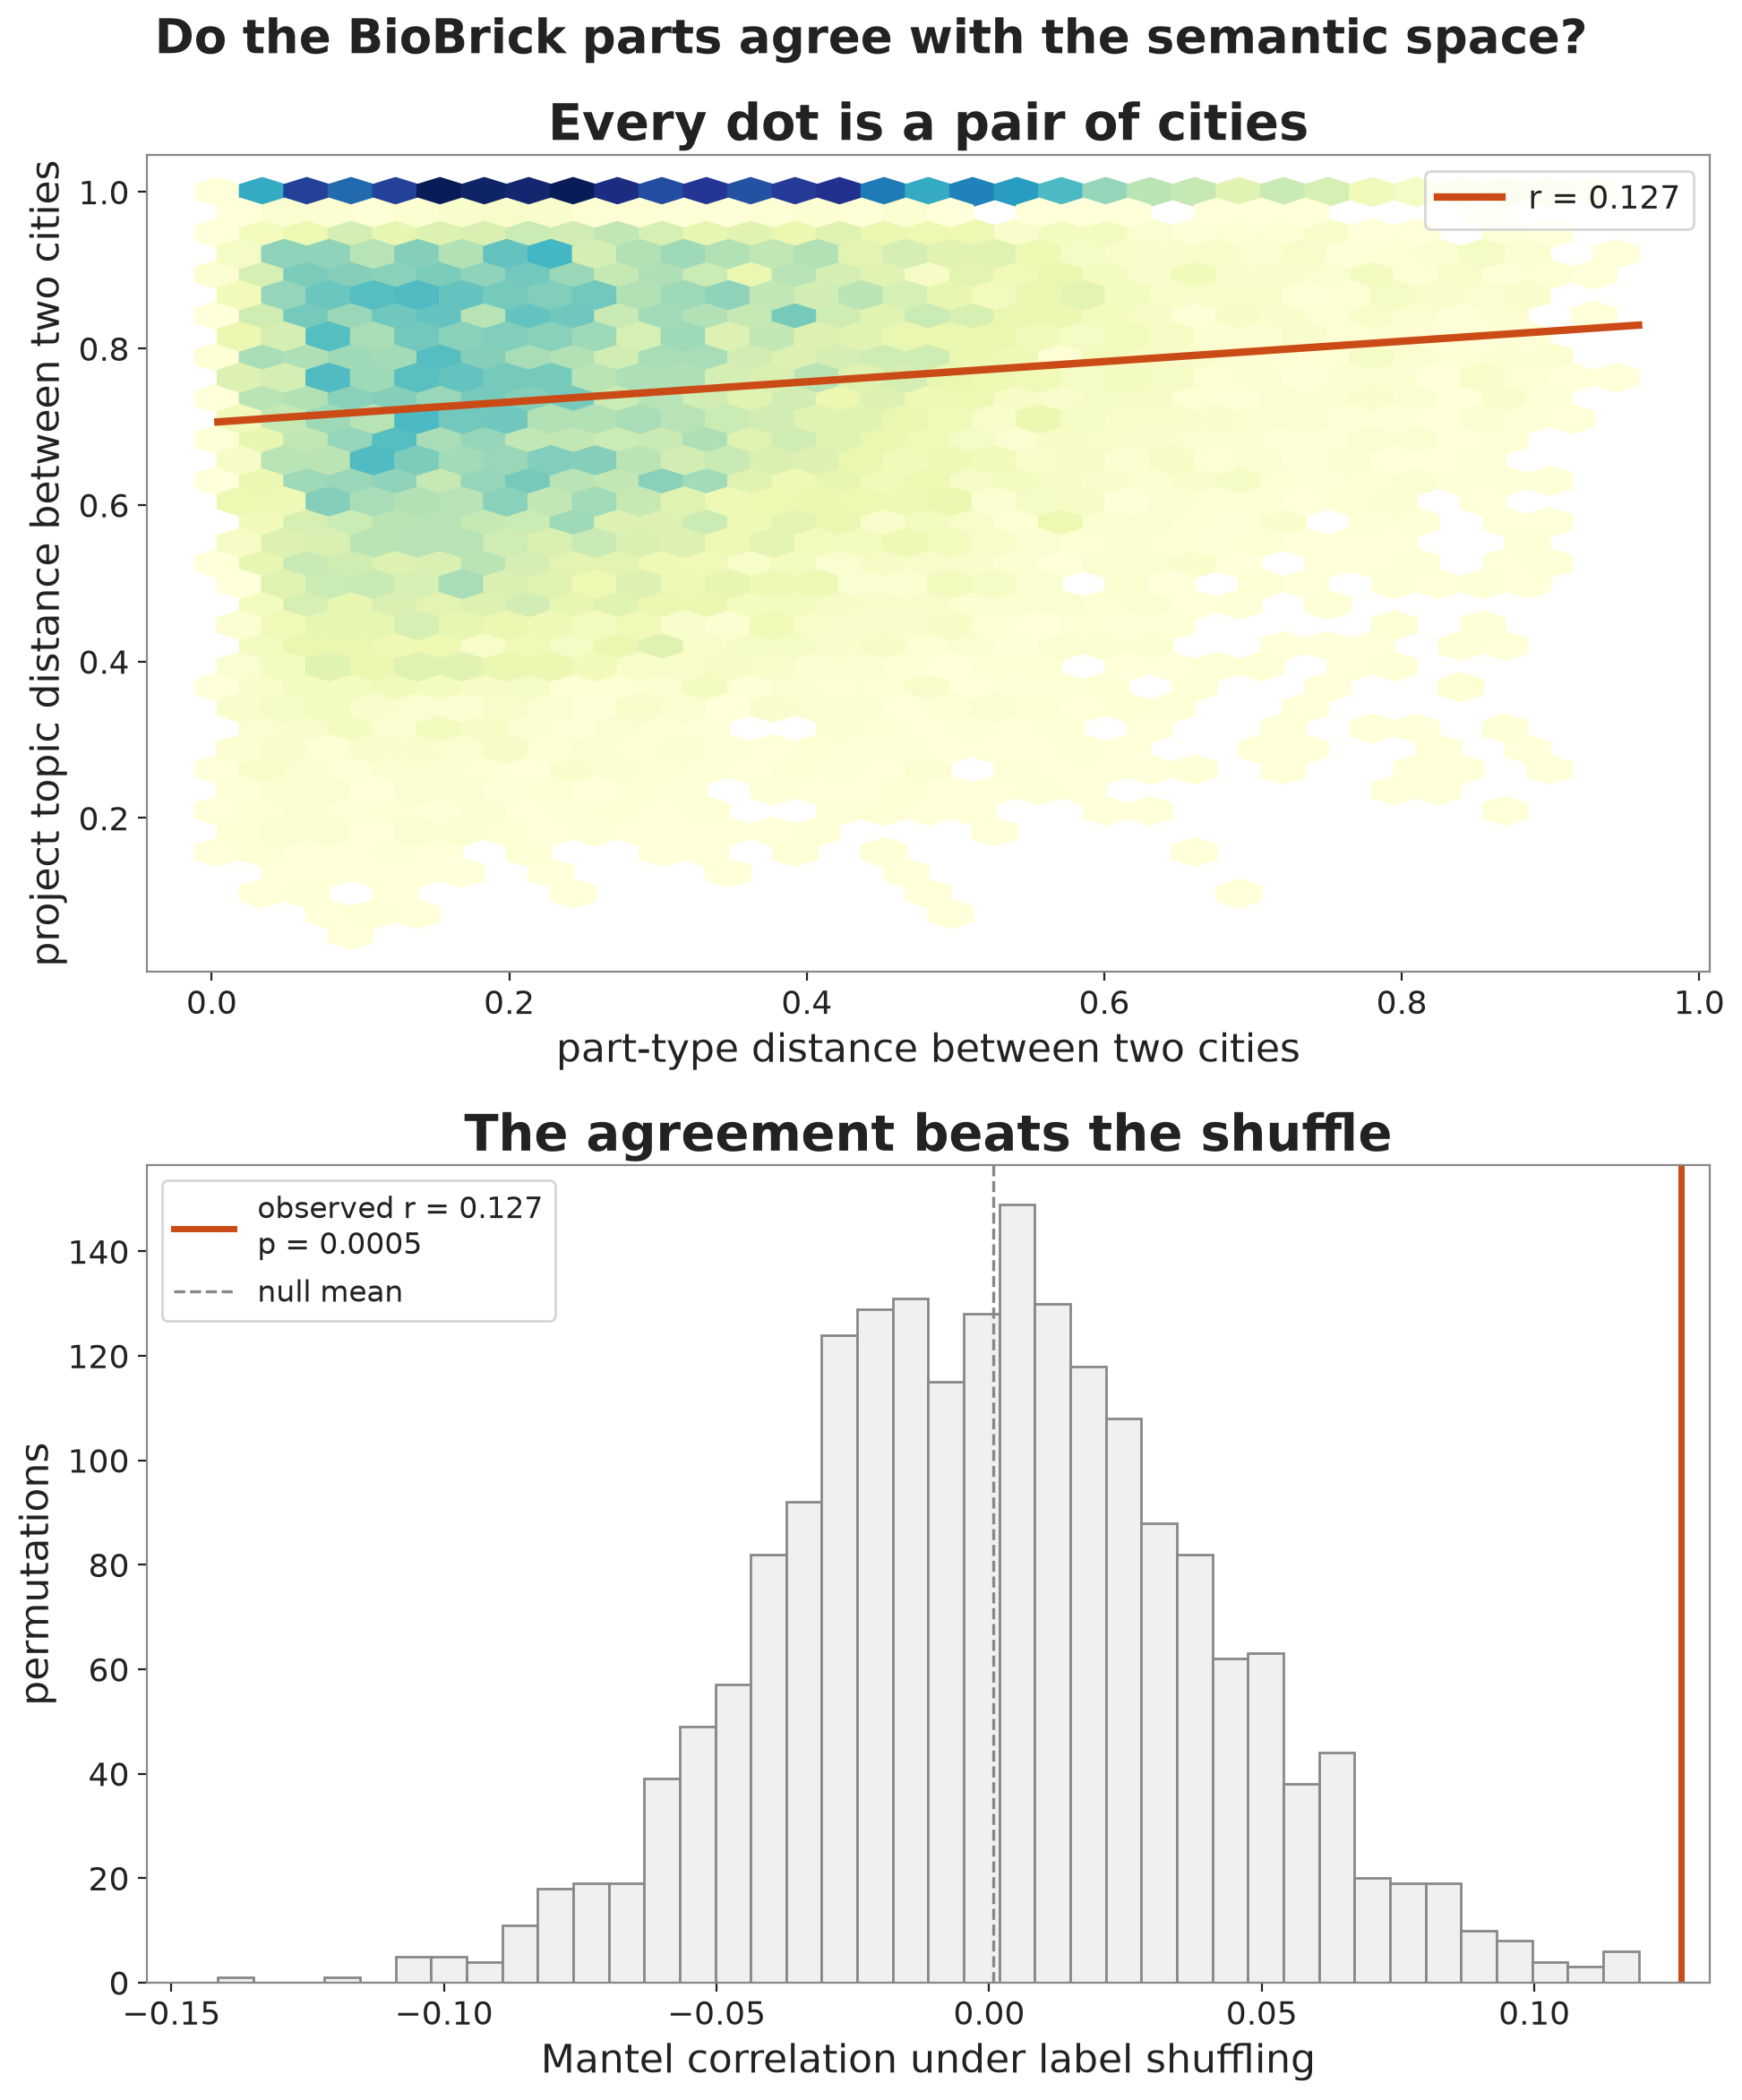
\includegraphics[width=0.85\linewidth]{mantel_parts_vs_topics.png}
\caption{Two independent views agree. City-pair similarity measured from the mix of BioBrick
part classes (never seen by the language model) correlates with city-pair similarity measured from semantic topic profiles. The relatedness is anchored outside the embedding space.}
\label{fig:mantel}
\end{figure}

The permutation behind the Mantel test confirms it is not a fluke: reshuffling the city labels thousands of times almost never produces a correlation this high by chance ($p = \statMantelP{}$). So the semantic relatedness is anchored to something outside itself. Two independent windows onto a city's synthetic biology, one made of words and one made of DNA parts, see the same shape. That is the strongest single piece of evidence in the thesis that the relatedness is real, and not a property of the tool used to measure it.

\subsection{Carbon-capture alignment}

Before asking which cities lead the carbon-capture work, it is worth checking that the general result applies to the case study specifically. The whole-corpus permutation test measures project-paper alignment across all of synthetic biology; if the carbon-capture subfield is a small, unusual corner of the data, the local alignment there could behave differently from the field-wide pattern. We ran the same project-level alignment analysis on the \statCcAlignN{} carbon-capture projects (those in clusters 7, 8, and 62), comparing each to papers in those clusters from the same city against papers in those clusters from other cities, across the \statCcAlignNCities{} cities with at least one carbon-capture project.

The carbon-capture alignment is as strong as the field-wide one. The mean alignment is $\bar{\delta}_{\text{CC}} = \statCcAlignMeanDelta{}$, with \statCcAlignFracPos{} of carbon-capture projects showing positive local alignment ($t = \statCcAlignTClustered{}$, clustered by city). The pattern is not a property of synthetic biology in general that dilutes when we focus on this subfield; it is at least as pronounced within carbon capture as across the whole corpus. The cities that matter for carbon capture are ones where the local alignment is real: their students and academics are not just both present in the subfield, but semantically closer to each other than to the global average of carbon-capture work. That specificity is what the city-level geography below is built on.

The last question narrows from the whole field to the carbon-capture case study, and from topics to specific places. The general result is about relatedness across many cities and many subfields; this section asks where the particular work on engineering microbes to capture carbon is concentrated, and whether the same cities appear across all three artifact types. The carbon-capture slice, clusters 7 (Cyanobacterial Metabolic Engineering), 8 (Cyanobacterial Chassis Development), and 62 (Industrial Fermentation), holds 452 artifacts across projects, papers, and patents, and they are not spread evenly. The clusters are themselves hierarchical: cluster 7 is dominated by student projects, cluster 8 by papers, and cluster 62 by patents, each representing a different face of the same technical activity. A city that appears across all three is one where the full chain, from student education to academic research to commercial filing, has taken root in a single place around a single theme. Those are the cities the policy question is really about.

To see the structure, we build a network of the carbon-capture artifacts and the links between them (Figure~\ref{fig:ccnet}). Nodes are projects, papers, and patents in the case-study clusters; edges are the concrete connections recovered in building the corpus, a project citing a paper, a paper naming a BioBrick, a patent paired with a paper it builds on. The result is not an even mesh. It has a backbone of well-connected documents surrounded by more loosely attached ones, and the cyanobacteria work forms a visibly distinct, tightly linked region. This is the carbon-capture story drawn as a graph: the Uppsala-style projects, the chassis-development papers, and the fermentation patents, wired together by the citations and parts that actually connect them.

\begin{figure}[htbp]
\centering
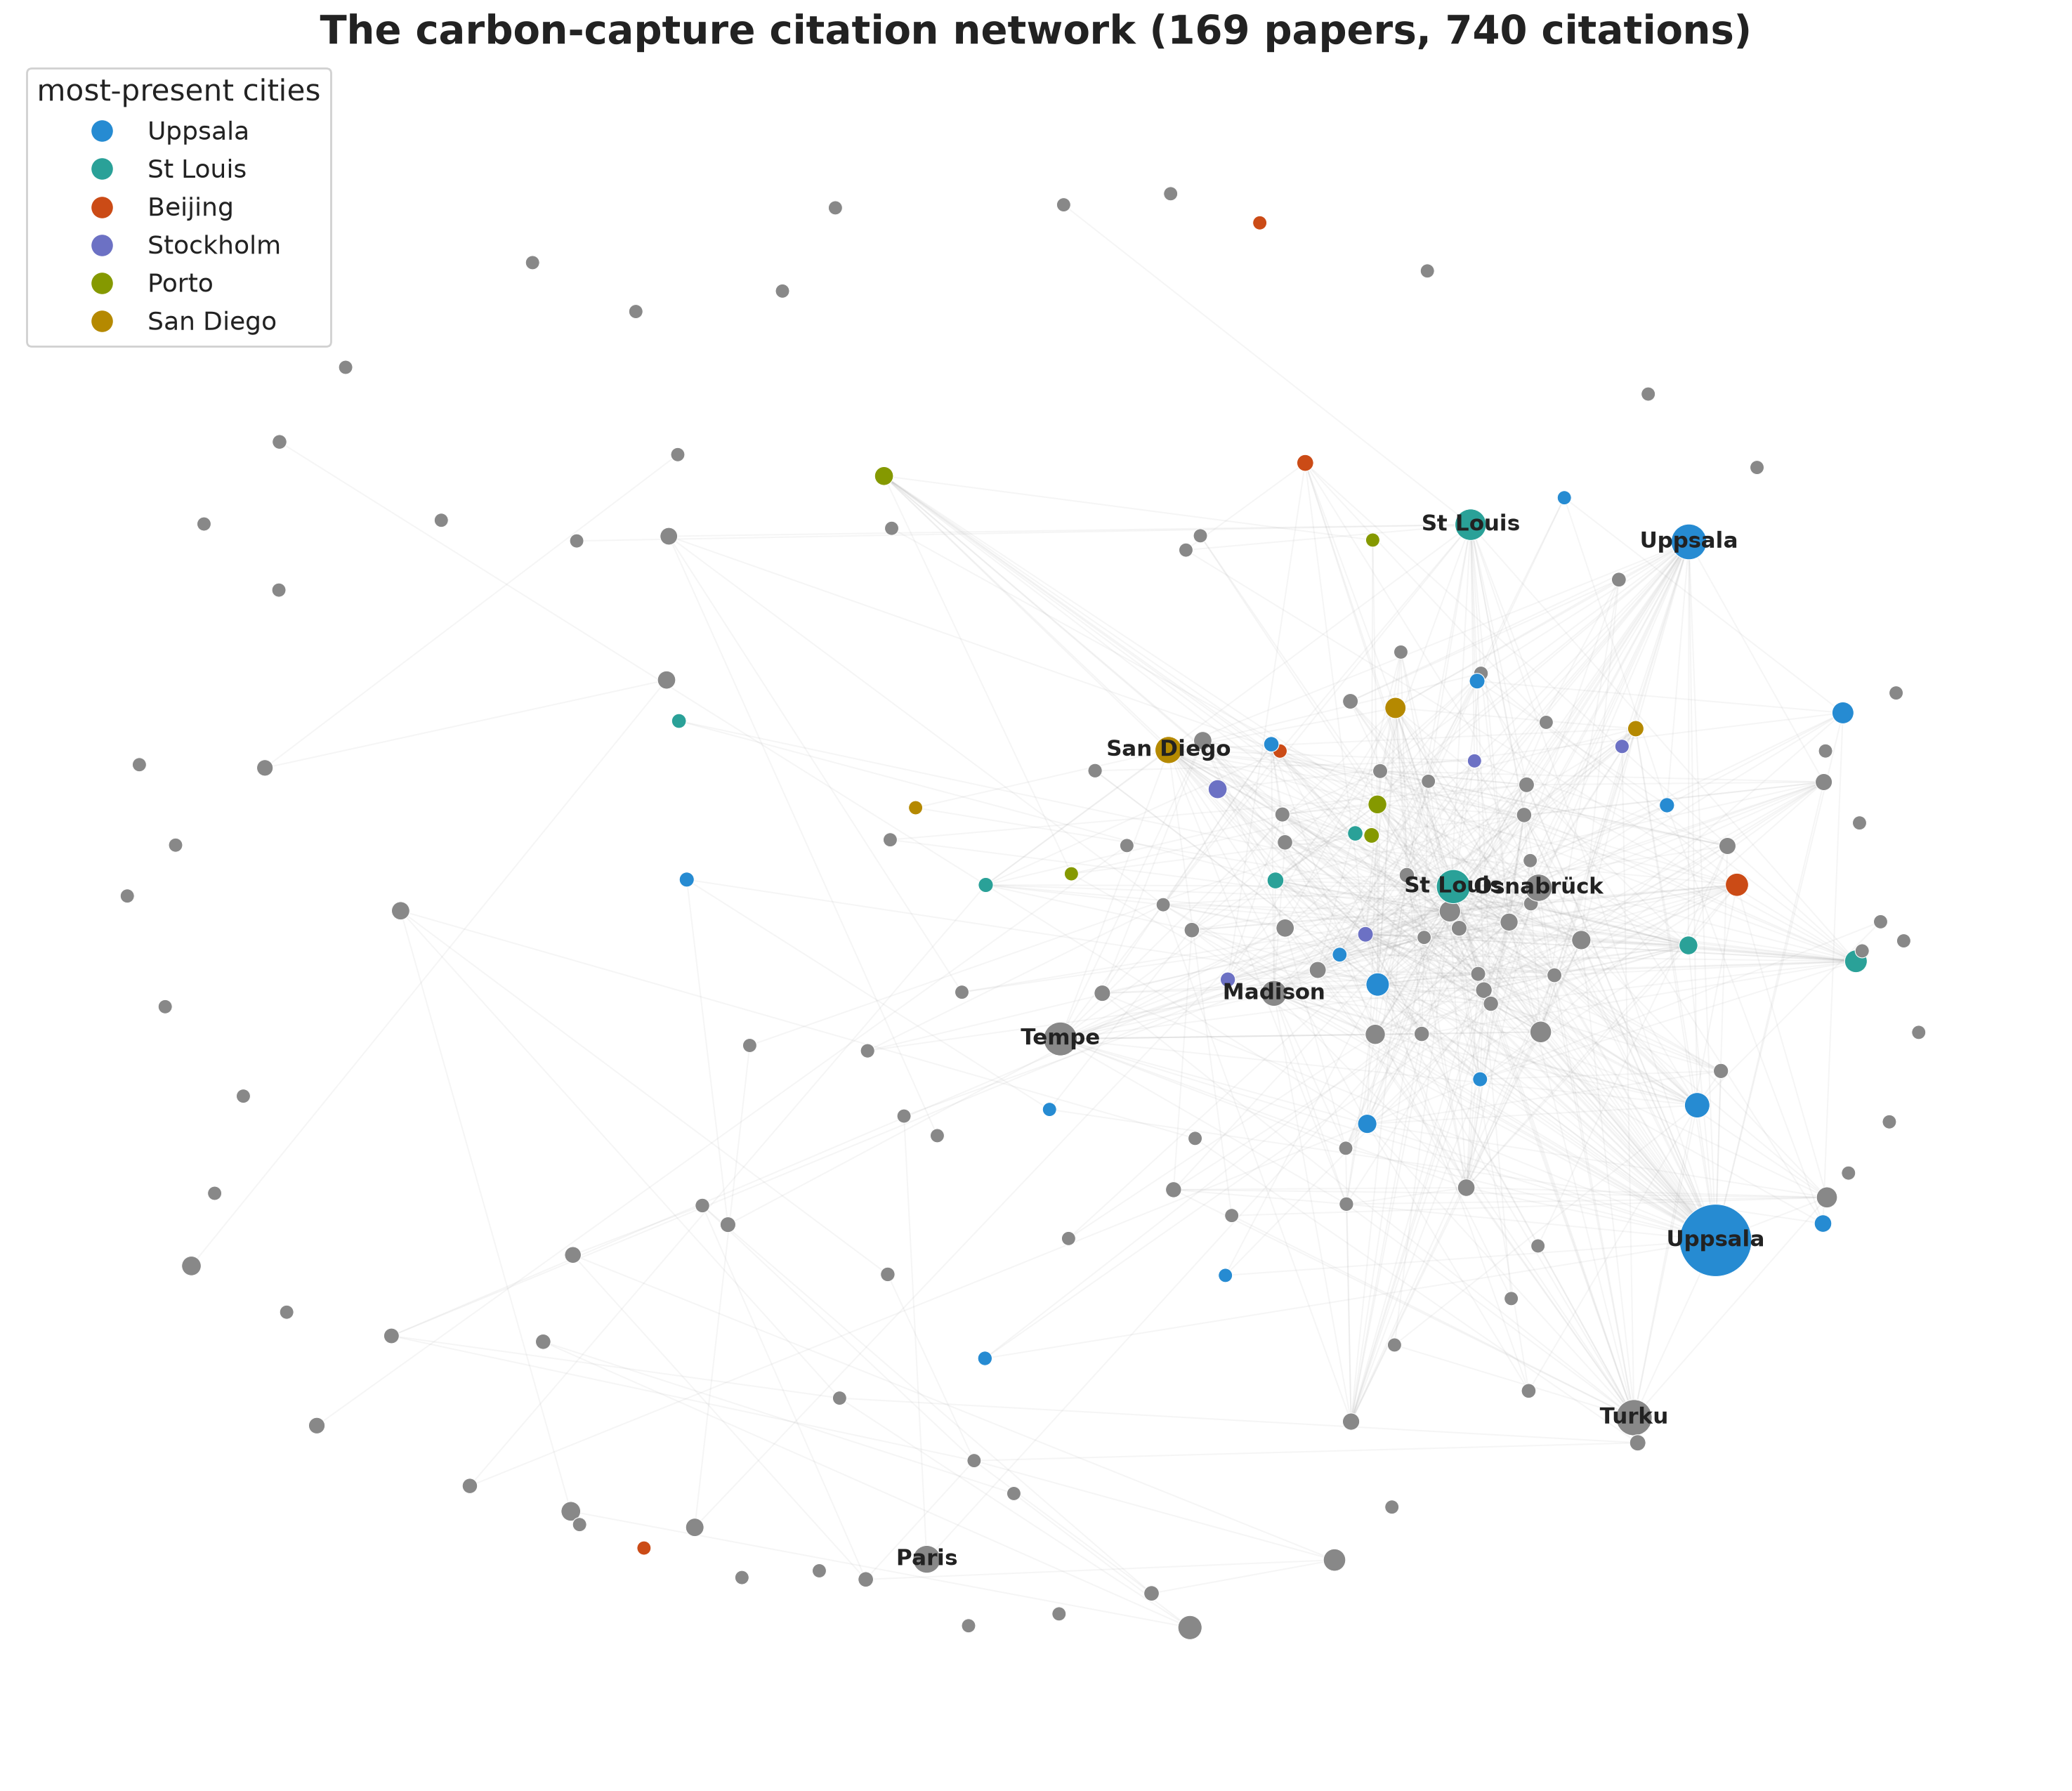
\includegraphics[width=0.85\linewidth]{cc_citation_network.png}
\caption{The carbon-capture network. Projects, papers, and patents in the case-study clusters,
linked by the citations and BioBrick connections recovered during corpus construction. The cyanobacterial work forms a distinct, tightly connected core.}
\label{fig:ccnet}
\end{figure}

A network lets us ask which cities are central in a precise sense. We aggregate the artifacts to their cities and measure each city's centrality, how well-connected its carbon-capture work is to everyone else's, not just how much of it there is (Figure~\ref{fig:cccentrality}). Volume and centrality usually travel together, but not always: a city can produce a lot of work that sits off on its own, or a little that is deeply wired into the rest. The cities that score high on centrality are the ones whose carbon-capture output is both substantial and connected, sitting on the paths between other cities' projects, papers, and patents. In this slice, a small group of cyanobacteria-focused cities dominates the measure.

\begin{figure}[htbp]
\centering

\includegraphics[width=0.85\linewidth]{cc_city_centrality.png}
\caption{City centrality in carbon capture. Cities ranked by how connected their
carbon-capture work is within the network, rather than by volume alone. Cyanobacteria-focused cities lead.}
\label{fig:cccentrality}
\end{figure}

Table~\ref{tab:cccities} lists the cities with the most carbon-capture artifacts across the three clusters, and the top of it is telling. Auckland and Uppsala lead, the two cities most heavily invested in engineering cyanobacteria to turn light and carbon dioxide into fuel, exactly the line of work \textit{Booze Bugs} began. Behind them come Daejeon, San Diego, and Gainesville, each a known centre of microbial and algal biotechnology. The list is not a ranking of who does carbon capture best; it is a map of where this specific line of synthetic biology has taken root across student, academic, and commercial work at once. If a policymaker asked where to look for cyanobacterial carbon capture, this table is a defensible first answer, and it was assembled from the bottom up, out of thousands of individual documents, without anyone deciding in advance which cities mattered.

\begin{table}[htbp]
\centering
\caption{Where cyanobacterial carbon capture has taken root. Cities with the most artifacts in
the carbon-capture clusters (7, Cyanobacterial Metabolic Engineering; 8, Cyanobacterial Chassis Development; 62, Industrial Fermentation), counting projects, papers, and patents together.}
\label{tab:cccities}
\begin{tabular}{lc}
\toprule
City & Carbon-capture artifacts \\
\midrule
Auckland & 19 \\
Uppsala & 18 \\
Daejeon & 15 \\
San Diego & 14 \\
Gainesville & 13 \\
Los Angeles & 9 \\
St Louis & 9 \\
Tianjin & 8 \\
\bottomrule
\end{tabular}
\end{table}

\subsection{Discussion}

Three bodies of literature give the results their interpretive frame, and it is worth placing each finding in the conversation that can use it.

The first is agglomeration and the geography of innovation. The core result, that a city's student projects and academic papers share specific research topics more than size and topic popularity can explain, is a new form of evidence for a familiar claim: that knowledge activity in a city is not a random sample of global output but a locally coherent specialization. The relatedness literature has established this for industries
\citep{hidalgoProductSpaceConditions2007}, for patents \citep{boschmaScientificKnowledgeDynamics2014},
and for scientific fields. This thesis extends the argument to a new type of actor. Student competitions had not previously been integrated into the city-level relatedness picture, and the positive result says they belong there. A city's iGEM teams are not an independent variable floating above the local research landscape; they are embedded in it, specializing in the same corners of the field where the academics and, further downstream, the patent filers concentrate. The Marshallian mechanism most consistent with this pattern is the labor-pooling and mentorship channel: the same faculty population advises students and runs labs, producing alignment through their shared topical interests. But the Jacobsian mechanism, the diverse city as a generator of novel combinations, is also operating, because the cities at the top of the leaderboard are large, diverse research hubs rather than narrow single-industry clusters.

The second conversation is the relatedness and proximity literature. Boschma's proximity framework \citep{boschmaProximityInnovationCritical2005} argues that productive knowledge interaction requires actors to be cognitively close as well as geographically proximate: sharing a neighborhood is necessary but not sufficient for knowledge exchange; sharing a knowledge base is what makes the exchange productive. The Jaccard topic overlap measure operationalizes cognitive proximity in a way that scales to a corpus spanning three artifact types: it asks not whether documents use the same words, but whether the actors that produced them invest in the same specific research clusters. The fact that this measure shows the excess that the centroid measure (a purer geographic proxy) obscures is precisely Boschma's point in empirical form: size and co-location create the potential for interaction, but cognitive alignment is what reveals whether that potential is being realized. The Mantel validation result — that the semantic topic distances between cities agree with the parts-class distances derived from entirely different data — confirms that the cognitive proximity picked up by the measure is anchored in something real, not in how the embedding model happens to organize text.

The third conversation is the Science of Science. Santolini and colleagues established iGEM as a model system for studying how teams collaborate and how network structure shapes scientific output \citep{santoliniIGEMModelSystem2023}. That work operates at the team level: which students worked with which advisors, and what did the network topology predict about project quality? The present thesis operates at the city level and adds a dimension that team-science studies typically omit: the commercial artifact. Papers and patents are both measured here, alongside the student projects, and the asymmetry in how the three relate is one of the more interesting findings. The project-to-paper link is strong; the paper-to-patent link is real; the direct project-to-patent link is the weakest of the three. This ladder structure, in which adjacent artifact types are more related than non-adjacent ones, is consistent with a model in which academic research is the translation layer that converts student work into commercial applications, rather than a world in which student ideas flow directly into patents. Whether that translation happens through career trajectories, through technology transfer, or through common mentors is a question the city-level data can suggest but not answer; individual-level matching of iGEM alumni to later patents would be required. The lead-lag result, a peak at $+3$ years, adds a temporal dimension to this: the Science of Science literature on how quickly academic knowledge becomes commercial typically operates at decade scales for patents; a three-year project-to-paper peak is notably fast, which may reflect the particular intensity and efficiency of the iGEM format as a research accelerator.

\subsection{Limitations}

A finding this specific comes with a specific set of limits, and they are worth stating together rather than scattered across earlier sections where they first arose.

The most consequential is the restriction to USPTO patents. We use US granted-patent records because they give every inventor a geocodable address, which no equivalent international database reliably provides. The practical result is that inventors who never filed in the United States are absent from the patent corpus entirely, which under-represents smaller national patent systems and systematically excludes work that was commercialized locally without a US filing. In principle this should not bias the project-paper alignment test, because the iGEM and OpenAlex corpora are international, but it does mean the patent leg of the three-way comparison is thinner for some cities than others. The alignment results should be read as project-to-paper alignment, with the patent-to-paper comparison supported by a less complete patent record.

The project corpus has its own coverage asymmetry. iGEM wikis are scraped from public URLs and are predominantly in English, which means teams whose documentation was written primarily in a language other than English may have shorter or lower-quality text fields, producing noisier embeddings for those projects. Chinese, Korean, and Central European teams are well represented in the roster but may be systematically under-represented in the text-based analysis if their English abstracts are brief. This would suppress the measured alignment for cities where those teams are concentrated, making the positive result again more conservative rather than inflated.

Geocoding introduces a third limitation. The multi-tier approach we used handles the vast majority of teams reliably, but the residual cases — teams resolved by a language model rather than by a registry lookup — carry a higher error rate. Geocoding errors place projects in the wrong city, which attenuates the city-level alignment test by injecting noise into the assignment of projects to their local paper environments. Any bias this creates runs against the positive result.

The corpus boundary itself is a limitation. The keyword strategy for OpenAlex papers trades recall for precision, and the Oldham patent set inherits whatever residual ambiguity exists at the field's edges. Some synthetic-biology documents are missed, and some adjacent documents are included. We have no way to estimate these error rates from the inside. The permutation test's null holds city size and topic popularity fixed and asks only whether the excess alignment is real given the corpus we have; it cannot address whether a different, better-bounded corpus would give a larger or smaller excess.

Finally, causal identification is beyond the reach of the current design. The corpus is observational, the geocoding is cross-sectional for patents, and the panel structure in the DiD rests on city-topic-period cells that are too aggregate for individual-level identification. We document a pattern; we do not identify the mechanism that produces it. The three candidate mechanisms described in the background, direct knowledge transfer, shared information environment, and student selection, all remain possible, and the data favor no single one. These limitations are not arguments against the finding, which survives its robustness checks; they are arguments about the scope of the claim. What the thesis establishes is real and size-independent; what it cannot establish is causal.

% ============================================================
\section{Conclusion}
% ============================================================

It has been a long route from the Anthropocene to a table of cities. The introduction opened with the observation that we have been reshaping the biosphere by accident, and asked whether the same tools could reshape it on purpose. The background placed that question inside a specific institutional structure: student competitions, academic labs, and commercial filers working in adjacent registers in the same cities, potentially connected into local innovation trajectories. The data chapter built the corpus that did not exist, resolving every ambiguity in the boundary of synthetic biology, the shape of iGEM's records, and the geography of three very different kinds of document. The results chapter asked the central question of the data directly, watched the first answer fail, understood why, replaced it with a measure that strips out the failure mode, and then spent the bulk of its length trying to break the answer it produced. What survived that treatment is what this conclusion claims.

The central claim is specific and modest: a city's iGEM projects and its academic papers share specific research topics more than size and topic popularity can explain, at a level of statistical confidence that a stringent permutation test places far beyond chance. That excess is not an artifact of one country, one cluster resolution, or one depth threshold. It is not a property of the embedding model, since it appears in the structure of the physical parts independently. And it is not merely a standing historical coincidence, since the difference-in-differences result finds a small but real year-to-year co-movement after each city's specialization is differenced out. The claim is well defended for what it is: a real, size-independent local alignment between student and academic synthetic biology.

Along the way the data drew a portrait of iGEM as more than a competition. It is a worldwide, open, standardized on-ramp into synthetic biology, and it leaves an unusually complete record: thousands of student projects, each tied to a place and a year, each built from a shared kit of parts that connect back to the literature and forward into new work. The Uppsala team turned sunlight into alcohol with blue-green algae, and two of its members carried that work into a research lab and a published paper that cited their own BioBrick. That thread, from a competition project to peer-reviewed science in the same city, is the whole thesis in miniature, and iGEM produces threads like it all over the world.

The central finding is specific, and it has a shape worth stating plainly. In a given city, the three artifact types are not equally related to one another. A city's patents are related to its papers, and its papers are related to its student projects, but its patents and its projects are the most distant of the three pairs. The chain is strongest between neighbours, project to paper and paper to patent, and weakest across the full span from student bench to commercial filing. That is what one would expect if ideas and capabilities travel in steps, with academic research as the middle link between student work and industry, though our data show the pattern, not the travel.

Read together, the results support a single narrative: student projects are embedded in the local research scene. Where a city's academics work, its students tend to work too, on the same specific topics, more than chance or size can explain, and the pattern is anchored in the physical parts the students build as much as in the words they write. That last point deserves emphasis. The BioBrick class distribution is a record of students' actual choices about what to build, made in a different register from any text the language model could have read. The fact that it agrees with the semantic topic structure confirms that the relatedness is about research orientation, not about a shared vocabulary that a text model might have imposed. The Mantel result is moderate in magnitude precisely because parts and text are two different views of the same underlying thing, not the same view described twice.

The difference-in-differences result adds a dynamic dimension to this picture. Most of the alignment is structural, a city's persistent concentration in particular subfields appearing simultaneously in its student and academic output, in the way that a city long invested in cyanobacterial research will produce both iGEM projects on cyanobacteria and publications on cyanobacteria, not necessarily because one causes the other, but because both draw on the same local ecosystem. But there is also a small year-to-year component: when a city's student projects lean into a topic in one period, its academic output in that topic rises slightly beyond its baseline, and vice versa. The coupling is not only historical; it is alive.

It bears repeating, because it is easy to forget in the momentum of a clean result: none of this is a causal claim. We have not shown that student projects cause later papers, or that academic work seeds student projects, or that either drives a patent. The three artifact types share many local causes: the same universities house student teams and research labs; the same mentors advise students and run labs; the same regional firms recruit from the same talent pool; the same funding agencies set priorities that shape what both students and academics choose to work on. Any or all of these common causes could produce the pattern we observe, with no direct flow of ideas from one artifact type to another required. We find relatedness and co-location; we cannot, from these data, separate that from a common environment that produces both.

The lead-lag result makes this point concrete. A peak at $+3$ years is consistent with the narrative that student projects precede academic papers in the same subfield, but it is also consistent with mentors who shift their focus from advising undergraduates to writing papers over a three-year research cycle, or with a city that responds to an external event in the two registers at different speeds. The correlation structure is exactly what a causal story would leave behind, which is why it is encouraging, but correlation structure alone cannot distinguish between causes. The data do what observational data can do: they document the pattern with enough rigor to rule out size and model artifacts as explanations. They do not rule out shared causes, and they are not designed to. Causal identification is a harder and different problem, requiring either a natural experiment or panel data on individuals, and it is one of the directions a follow-up should take.

That limit is also an invitation. The relatedness we document is exactly the pattern a causal story would leave behind, which makes it a solid foundation for work designed to test one. Tracing named individuals from iGEM rosters into later authorships and patents, or following specific parts from the registry into commercial filings, could turn co-location into something closer to a trajectory. This thesis maps the ground; it does not yet walk the path across it.

There are several such paths, left unwalked mostly for want of time. A master's thesis has a fixed horizon, and a number of the richest questions sit just past it.

The wiki citations we scraped offer a first extension. Many iGEM teams cite specific academic papers in their project documentation; we used those citations as fine-tuning links rather than incorporating all the cited papers into the main corpus. A full network built from those citations would let us ask a more precise version of the geographic question: do iGEM teams cite researchers from their own city more than chance predicts? Citation locality in the academic literature has been documented \citep{breschiKnowledgeSpilloversLocal2001}, but the pattern among students is unstudied, and the directionality would be informative. A team that over-cites local academics is drawing on local knowledge; a team that cites globally is connected to a broader network. Both patterns would tell us something about how the local ecosystem operates.

The Marx patent-paper pairs were used in partial form for fine-tuning but could be reproduced in full for a more complete analysis of the paper-to-patent link. We did not have the computational resources to run the full matching pipeline; doing so would substantially thicken the patent-to-paper edges and allow a more precise test of whether the academic work is specifically local to the same city as the patent, or whether academic-to-patent transfer is less geographically sticky than the project-to-paper link. The data are public; the pipeline is documented in the literature; this is primarily a question of compute and time.

The most ambitious extension would follow named individuals. The iGEM roster is a list of students and their institutions, going back to 2004; academic authorship records are largely public; patent inventor lists name individuals with addresses. Linking these three records would allow career trajectory analysis at a level of resolution that no existing iGEM study has achieved. The competition's own track record of producing founders, postdocs, and senior researchers is well known anecdotally but poorly documented systematically. A matched panel that follows iGEM alumni into authorship and patents could finally put numbers on it.

The fine-tuned model is itself a reusable product. We adapted SPECTER2 into an embedding that places synthetic biology's projects, papers, patents, and parts in one space, and that space is useful beyond the questions asked here. It could power a semantic search tool for the field: give it a project idea, a patent, or a genetic part, and it returns the related work of every type, across the boundaries that keyword search and citation databases cannot cross. For a student planning an iGEM project, a researcher scanning for prior art, or a funder mapping a field, a search that reads meaning across artifact types would be worth having. The model is on the public repository, ready to build on.

For anyone whose interest is narrower and more practical, the case study points somewhere specific. If you want to work on engineering cyanobacteria to capture carbon, the data says Uppsala and Auckland are the places to be. They sit at the top of the carbon-capture leaderboard and at the centre of its network, cities where student projects, academic papers, and commercial patents on blue-green algae have all taken root together. The concentration is not an accident of one dataset; it is where a genuine local specialization has formed.

One unfinished thread is worth flagging because it is so promising. Many patents contain digitized genetic sequences, the actual DNA of the invention, and services like Lens.org's PatSeq make that data searchable. Acquiring it at scale was beyond this project's budget, but the idea it enables is striking: search the sequences of academic and commercial work directly, and see whether BioBrick sequences from the student registry show up in later patent filings. One could embed patent abstracts in one space and their genetic sequences in another, using a sequence model in place of a language one, and ask whether the two spaces agree, the same cross-modal validation we ran with parts, but at the level of DNA itself. Tracing individual sequences of genetic code through the knowledge space is a study waiting to be done.

Step back, and a policy point comes into focus. These ecosystems, student, academic, and commercial, are deeply intertwined; they share cities, mentors, methods, and, as we have shown, topics. Student projects are an early, legible layer of that ecosystem, forming in the same places and on the same subjects as the research and industry around them. If a city's iGEM teams are a visible early signal of where its synthetic biology is heading, then supporting them, and the open science they practice, is a low-cost way of investing in a field's future. Governments looking to seed emerging technologies could do worse than to fund the students already teaching themselves to build them.

There is a larger stake under all of this. The tools that let us read and write life are getting cheaper and more powerful every year, and they are spreading into the hands of students. The same capability could deepen the damage of the Anthropocene or help repair it; the algae that once remade the atmosphere by accident are now being engineered, on purpose, to pull carbon back out of it. Which future we get is not settled, and it will be shaped by who learns to hold the pen and what they choose to write. Science fiction has quietly become science fact. The generation now turning sunlight into fuel for a competition is the one that will decide what this technology is for. That is worth watching closely, and worth investing in, because the future it is drafting is the one the rest of us will live in.

\bibliographystyle{plainnat}
\bibliography{references,references_extra}

\end{document}
